\documentclass{beamer}
% =============================================================================
% ENCODING
% =============================================================================
\usepackage[utf8]{inputenc}  % UTF-8 encoding support

% =============================================================================
% GRAPHICS
% =============================================================================
\usepackage{graphicx}  % For \includegraphics (401 uses across lectures)

% =============================================================================
% MATH PACKAGES
% =============================================================================
\usepackage{amsmath}    % For align, multline, equation environments (heavily used)
\usepackage{amsfonts}   % For \mathbb (e.g., \bbR, \bbE)
\usepackage{amssymb}    % For additional math symbols

% =============================================================================
% TABLES
% =============================================================================
\usepackage{booktabs}   % For \toprule, \midrule, \bottomrule (used in lecture13, lecture14)

% =============================================================================
% LISTS
% =============================================================================
\usepackage{enumerate}  % Enhanced enumerate environment (76 uses across lectures)

% =============================================================================
% TIKZ (DIAGRAMS)
% =============================================================================
\usepackage{tikz}       % For taxonomy diagram and footnotes positioning

% =============================================================================
% UTILITY PACKAGES
% =============================================================================
\usepackage{multido}    % For \multido command used in \eqpause
\usepackage{etoolbox}   % For \AtEndEnvironment, \ifbool, \newbool (used in preamble and taxonomy)
\usepackage{xspace}     % For smart spacing after custom commands (\ODESolve, \SDESolve)

% =============================================================================
% BEAMER THEME SETTINGS
% =============================================================================
\usetheme{default}
\usecolortheme{default}

\setbeamerfont{title}{size=\Huge}
\setbeamertemplate{footline}[frame number]{}
\setbeamertemplate{section in toc}[sections numbered]

\makeatletter
\newcommand\HUGE{\@setfontsize\Huge{35}{40}}
\makeatother    

\setbeamerfont{title}{size=\HUGE}
\beamertemplatenavigationsymbolsempty

% =============================================================================
% TIKZ LIBRARIES
% =============================================================================
% Used for taxonomy diagram: arrows, positioning, shapes
\usetikzlibrary{arrows.meta,calc,shapes,positioning,shadows,trees}

% =============================================================================
% CUSTOM FOOTNOTE COMMANDS
% =============================================================================
% \myfootnote{text} - creates a footnote at the bottom of the slide
\newcommand\myfootnote[1]{%
  \vspace{-0.5cm}%
  \tikz[remember picture,overlay]
  \draw (current page.south west) +(1in + \oddsidemargin,0.5em)
  node[anchor=south west,inner sep=0pt]{\parbox{\textwidth}{%
      \rlap{\rule{10em}{0.4pt}}\raggedright\scriptsize \textit{#1}}};}

% \myfootnotewithlink{url}{text} - creates a clickable footnote (623 uses across lectures)
\newcommand\myfootnotewithlink[2]{%
  \vspace{-0.5cm}%
  \tikz[remember picture,overlay]
  \draw (current page.south west) +(1in + \oddsidemargin,0.5em)
  node[anchor=south west,inner sep=0pt]{\parbox{\textwidth}{%
      \rlap{\rule{10em}{0.4pt}}\raggedright\scriptsize\href{#1}{\textit{#2}}}};}

% =============================================================================
% SECTION/SUBSECTION OUTLINE AUTOMATION
% =============================================================================
% Automatically show outline at the beginning of each section
\AtBeginSection[]
      {
      	\begin{frame}{Outline}
      		\tableofcontents[currentsection]
      	\end{frame}
      }
      \AtBeginSubsection[]{
      	\begin{frame}{Outline}
      		\tableofcontents[currentsection,currentsubsection]
      	\end{frame}
}

% =============================================================================
% CUSTOM SLIDE ANIMATION COMMANDS
% =============================================================================
% These commands enable step-by-step reveal of equations and content
% Used heavily across all lectures (1130+ uses of \nextonslide and \eqpause)

\newcounter{noscounter}   % Counter for \nextonslide (resets on each new slide)
\newcounter{pcounter}     % Counter for pause commands (resets after \eqpause)
\newcounter{diffcounter}  % Counts pauses after equations

% \nextonslide{content} - reveals content on the next overlay
\newcommand{\nextonslide}[1]{%
  \stepcounter{noscounter}%
  \stepcounter{pcounter}%
  \stepcounter{diffcounter}%
  \onslide<\value{noscounter}->{#1}%
}

% \resetonslide - resets all animation counters (called at each frame)
\newcommand{\resetonslide}{%
    \setcounter{noscounter}{1}%
    \setcounter{pcounter}{1}%
    \setcounter{diffcounter}{0}%
}

% \eqpause - pause after equation that syncs with \nextonslide
\newcommand{\eqpause}{%
  \multido{\i=1+1}{\value{pcounter}}{\pause}%
  \stepcounter{noscounter}%
  \setcounter{pcounter}{1}%
}

% \eqpausediff - helper command, runs automatically after math environments
\newcommand{\eqpausediff}{%
  \multido{\i=1+1}{\value{diffcounter}}{\pause}%
  \addtocounter{pcounter}{-\value{diffcounter}}%
  \setcounter{diffcounter}{0}%
}

% Apply \eqpausediff after math environments
\newcommand\AtEndBoth[2]{%
  \AtEndEnvironment{#1}{#2}%
  \AtEndEnvironment{#1*}{#2}%
}

\AtEndBoth{align}{\eqpausediff}
\AtEndBoth{equation}{\eqpausediff}
\AtEndBoth{multline}{\eqpausediff}

% Reset counters at the beginning of each frame
\addtobeamertemplate{frametitle}{\resetonslide}{}

% =============================================================================
% INCLUDE OTHER CONFIGURATION FILES
% =============================================================================
% ==============================================================================
% Custom LaTeX Commands for Deep Generative Models Course
% ==============================================================================

% ==============================================================================
% BOLD LETTERS (mathbf / boldsymbol)
% ==============================================================================

% ------------------------------------------------------------------------------
% Latin Bold Lowercase
% Usage: \bx for x in bold, commonly used for vectors
% ------------------------------------------------------------------------------
\newcommand{\ba}{\mathbf{a}}
\newcommand{\bc}{\mathbf{c}}
\newcommand{\be}{\mathbf{e}}
\newcommand{\bff}{\mathbf{f}}  % Note: \bf is reserved for bold font switching
\newcommand{\bg}{\mathbf{g}}
\newcommand{\bh}{\mathbf{h}}
\newcommand{\bp}{\mathbf{p}}
\newcommand{\bq}{\mathbf{q}}
\newcommand{\bs}{\mathbf{s}}
\newcommand{\bt}{\mathbf{t}}
\newcommand{\bu}{\mathbf{u}}
\newcommand{\bv}{\mathbf{v}}
\newcommand{\bw}{\mathbf{w}}
\newcommand{\bx}{\mathbf{x}}
\newcommand{\by}{\mathbf{y}}
\newcommand{\bz}{\mathbf{z}}
\newcommand{\bzero}{\boldsymbol{0}}  % Zero vector
\newcommand{\bone}{\mathbf{1}}       % Ones vector

% ------------------------------------------------------------------------------
% Latin Bold Uppercase
% Usage: \bX for X in bold, commonly used for matrices or random vectors
% ------------------------------------------------------------------------------
\newcommand{\bA}{\mathbf{A}}
\newcommand{\bG}{\mathbf{G}}
\newcommand{\bI}{\mathbf{I}}
\newcommand{\bJ}{\mathbf{J}}
\newcommand{\bL}{\mathbf{L}}
\newcommand{\bM}{\mathbf{M}}
\newcommand{\bP}{\mathbf{P}}
\newcommand{\bQ}{\mathbf{Q}}
\newcommand{\bR}{\mathbf{R}}
\newcommand{\bT}{\mathbf{T}}
\newcommand{\bU}{\mathbf{U}}
\newcommand{\bV}{\mathbf{V}}
\newcommand{\bW}{\mathbf{W}}
\newcommand{\bX}{\mathbf{X}}
\newcommand{\bZ}{\mathbf{Z}}

% ------------------------------------------------------------------------------
% Greek Bold Lowercase
% Usage: \btheta for θ in bold, commonly used for parameter vectors
% ------------------------------------------------------------------------------
\newcommand{\bepsilon}{\boldsymbol{\epsilon}}
\newcommand{\blambda}{\boldsymbol{\lambda}}
\newcommand{\bmu}{\boldsymbol{\mu}}
\newcommand{\bphi}{\boldsymbol{\phi}}
\newcommand{\bpi}{\boldsymbol{\pi}}
\newcommand{\bpsi}{\boldsymbol{\psi}}
\newcommand{\bsigma}{\boldsymbol{\sigma}}
\newcommand{\btheta}{\boldsymbol{\theta}}

% ------------------------------------------------------------------------------
% Greek Bold Uppercase
% Usage: \bSigma for Σ in bold, commonly used for covariance matrices
% ------------------------------------------------------------------------------
\newcommand{\bPhi}{\boldsymbol{\Phi}}
\newcommand{\bSigma}{\boldsymbol{\Sigma}}
\newcommand{\bTheta}{\boldsymbol{\Theta}}

% ==============================================================================
% CALLIGRAPHIC LETTERS (mathcal)
% Usage: \cX for calligraphic X, commonly used for sets and spaces
% ==============================================================================
\newcommand{\cF}{\mathcal{F}}
\newcommand{\cI}{\mathcal{I}}
\newcommand{\cL}{\mathcal{L}}
\newcommand{\cM}{\mathcal{M}}
\newcommand{\cN}{\mathcal{N}}
\newcommand{\cO}{\mathcal{O}}
\newcommand{\cP}{\mathcal{P}}
\newcommand{\cS}{\mathcal{S}}
\newcommand{\cT}{\mathcal{T}}
\newcommand{\cW}{\mathcal{W}}
\newcommand{\cX}{\mathcal{X}}
\newcommand{\cZ}{\mathcal{Z}}

% ==============================================================================
% BLACKBOARD BOLD LETTERS (mathbb)
% Usage: \bbR for ℝ, commonly used for number sets and expectations
% ==============================================================================
\newcommand{\bbE}{\mathbb{E}}  % Expectation
\newcommand{\bbI}{\mathbb{I}}  % Indicator function
\newcommand{\bbP}{\mathbb{P}}  % Probability measure
\newcommand{\bbR}{\mathbb{R}}  % Real numbers

% ==============================================================================
% MATH OPERATORS
% ==============================================================================

% ------------------------------------------------------------------------------
% Optimization Operators
% Usage: \argmin_{x} f(x) for proper spacing and limits placement
% ------------------------------------------------------------------------------
\DeclareMathOperator*{\argmin}{arg\,min}
\DeclareMathOperator*{\argmax}{arg\,max}

% ------------------------------------------------------------------------------
% Statistical Operators
% Usage: \cov(X, Y) for covariance
% ------------------------------------------------------------------------------
\DeclareMathOperator{\cov}{cov}

% ------------------------------------------------------------------------------
% Linear Algebra Operators
% Usage: \tr(\bA) for trace of matrix A
% ------------------------------------------------------------------------------
\DeclareMathOperator{\tr}{tr}

% ------------------------------------------------------------------------------
% Other Mathematical Operators
% ------------------------------------------------------------------------------
\DeclareMathOperator{\diver}{div}      % Divergence (vector calculus)
\newcommand{\sg}{\mathrm{sg}}          % Stop-gradient operator
\DeclareMathOperator{\softmax}{softmax}
\DeclareMathOperator{\supp}{supp}      % Support of a distribution

% ==============================================================================
% PROBABILITY DISTRIBUTIONS
% Usage: X \sim \cN(0, 1), Y \sim \Bern(p)
% ==============================================================================
\DeclareMathOperator{\Bern}{Bern}      % Bernoulli distribution
\DeclareMathOperator{\Cat}{Cat}        % Categorical distribution
\DeclareMathOperator{\Gumbel}{Gumbel}  % Gumbel distribution
\DeclareMathOperator{\Uniform}{Uniform}

% ==============================================================================
% METRICS AND DIVERGENCES
% Usage: \KL(p \| q), \JSD(p, q)
% ==============================================================================
\newcommand{\Ent}{\mathrm{H}}          % Entropy
\newcommand{\FID}{\mathrm{FID}}        % Fréchet Inception Distance
\newcommand{\JSD}{D_\mathrm{JS}}        % Jensen-Shannon Divergence
\newcommand{\KL}{D_\mathrm{KL}}        % Kullback-Leibler Divergence
\DeclareMathOperator{\MMD}{MMD}        % Maximum Mean Discrepancy
\DeclareMathOperator{\SNR}{SNR}        % Signal-to-Noise Ratio

% ==============================================================================
% NEURAL NETWORK NOTATION
% ==============================================================================

% ------------------------------------------------------------------------------
% Network Architectures (upright font for abbreviations)
% Usage: f_{\btheta} = \NN_{\btheta}(\bx)
% ------------------------------------------------------------------------------
\newcommand{\MLP}{\mathrm{MLP}}        % Multi-Layer Perceptron
\newcommand{\NN}{\mathrm{NN}}          % Neural Network
\newcommand{\RNN}{\mathrm{RNN}}        % Recurrent Neural Network

% ------------------------------------------------------------------------------
% Numerical Solvers (monospace font)
% Usage: \bx_T = \ODESolve(v, \bx_0, T)
% ------------------------------------------------------------------------------
\newcommand{\ODESolve}{\texttt{ODESolve}\xspace}
\newcommand{\SDESolve}{\texttt{SDESolve}\xspace}

% ==============================================================================
% COMMON SHORTCUTS
% Usage: Frequently used subscripted or parameterized expressions
% ==============================================================================
\newcommand{\pd}{p_{\text{data}}}              % Data distribution
\newcommand{\pt}{p_{\boldsymbol{\theta}}}      % Parameterized distribution
\newcommand{\qagg}{q_{\text{agg}}}             % Aggregated posterior
\newcommand{\lambdamax}{\lambda_{\text{max}}}  % Maximum eigenvalue
  % Math shorthand commands (\bx, \bbE, \KL, etc.)
\input{../utils/title}        % Title page template
% For each possible node, we create a boolean
\newbool{hl@root}
\newbool{hl@explicit}
\newbool{hl@implicit}
\newbool{hl@exact}
\newbool{hl@approx}
\newbool{hl@gan}
\newbool{hl@ar}
\newbool{hl@nf}
\newbool{hl@vae}
\newbool{hl@score}
\newbool{hl@cont}
\newbool{hl@ddpm}
\newbool{hl@sm}
\newbool{hl@ode}
\newbool{hl@sde}
\newbool{hl@fm}

% Command to reset all bools
\newcommand{\resetAllHighlights}{%
    \boolfalse{hl@root}%
    \boolfalse{hl@explicit}%
    \boolfalse{hl@implicit}%
    \boolfalse{hl@exact}%
    \boolfalse{hl@approx}%
    \boolfalse{hl@gan}%
    \boolfalse{hl@ar}%
    \boolfalse{hl@nf}%
    \boolfalse{hl@vae}%
    \boolfalse{hl@score}%
    \boolfalse{hl@cont}%
    \boolfalse{hl@ddpm}%
    \boolfalse{hl@sm}%
    \boolfalse{hl@ode}%
    \boolfalse{hl@sde}%
    \boolfalse{hl@fm}%
}

% Command to set a single highlight
\newcommand{\setHighlight}[1]{%
    \booltrue{hl@#1}%
}

% Command to set highlights from comma-separated list
\newcommand{\setHighlights}[1]{%
    \resetAllHighlights%
    \forcsvlist{\setHighlight}{#1}%
}

% Highlighted style definition
\tikzset{
    hl/.style={line width=1.2pt, draw=black, font=\scriptsize\bfseries},
    box/.style={
        rectangle, 
        draw=gray!50, 
        rounded corners=2pt, 
        minimum width=1.9cm, 
        minimum height=0.5cm, 
        align=center, 
        font=\scriptsize, 
        line width=0.4pt
    },
    rootnode/.style={box, fill=violet!20},
    category/.style={box, fill=teal!20},
    model/.style={box, fill=yellow!30},
    arrow/.style={-Stealth, draw=gray!80, line width=0.4pt}
}

% Draw taxonomy with pre-set highlights
\newcommand{\drawTaxonomy}{%
    \begin{tikzpicture}[scale=0.9, transform shape, node distance=0.6cm and 0.3cm]
        % --- CENTRAL ROOT ---
        \ifbool{hl@root}{\node[rootnode, hl] (root) {Generative Models};}{\node[rootnode] (root) {Generative Models};}

        % --- UPPER BRANCHES ---
        \ifbool{hl@explicit}{\node[category, hl, above left=0.6cm and 0.5cm of root] (explicit) {Explicit density};}{\node[category, above left=0.6cm and 0.5cm of root] (explicit) {Explicit density};}
        \ifbool{hl@implicit}{\node[category, hl, above right=0.6cm and 0.5cm of root] (implicit) {Implicit density};}{\node[category, above right=0.6cm and 0.5cm of root] (implicit) {Implicit density};}

        \ifbool{hl@exact}{\node[category, hl, above left=0.6cm and -0.6cm of explicit] (exact) {Exact likelihood};}{\node[category, above left=0.6cm and -0.6cm of explicit] (exact) {Exact likelihood};}
        \ifbool{hl@approx}{\node[category, hl, above right=0.6cm and -0.6cm of explicit] (approx) {Approximate likelihood};}{\node[category, above right=0.6cm and -0.6cm of explicit] (approx) {Approximate likelihood};}

        \ifbool{hl@gan}{\node[model, hl, above=0.6cm of implicit] (gans) {GANs};}{\node[model, above=0.6cm of implicit] (gans) {GANs};}

        \ifbool{hl@ar}{\node[model, hl, above left=0.6cm and -0.9cm of exact] (ar) {Autoregressive \\ models};}{\node[model, above left=0.6cm and -0.9cm of exact] (ar) {Autoregressive \\ models};}
        \ifbool{hl@nf}{\node[model, hl, above right=0.6cm and -0.9cm of exact] (nf) {Normalizing \\ Flows};}{\node[model, above right=0.6cm and -0.9cm of exact] (nf) {Normalizing \\ Flows};}
        \ifbool{hl@vae}{\node[model, hl, above=0.6cm of approx] (vae) {Variational \\ Autoencoders};}{\node[model, above=0.6cm of approx] (vae) {Variational \\ Autoencoders};}

        % --- LOWER BRANCHES ---
        \ifbool{hl@score}{\node[category, hl, below left=0.6cm and 0.5cm of root] (score) {Score-based};}{\node[category, below left=0.6cm and 0.5cm of root] (score) {Score-based};}
        \ifbool{hl@cont}{\node[category, hl, below right=0.6cm and 0.5cm of root] (cont) {Continuous \\ dynamics};}{\node[category, below right=0.6cm and 0.5cm of root] (cont) {Continuous \\ dynamics};}

        \ifbool{hl@sm}{\node[model, hl, below left=0.6cm and -0.8cm of score] (sm) {Score Matching};}{\node[model, below left=0.6cm and -0.8cm of score] (sm) {Score Matching};}
        \ifbool{hl@ddpm}{\node[model, hl, below right=0.6cm and -0.8cm of score] (ddpm) {Denoising Diffusion};}{\node[model, below right=0.6cm and -0.8cm of score] (ddpm) {Denoising Diffusion};}

        \ifbool{hl@ode}{\node[model, hl, below left=0.6cm and -0.8cm of cont] (ode) {Neural ODEs};}{\node[model, below left=0.6cm and -0.8cm of cont] (ode) {Neural ODEs};}
        \ifbool{hl@sde}{\node[model, hl, below right=0.6cm and -0.8cm of cont] (sde) {SDE-based \\ Diffusion};}{\node[model, below right=0.6cm and -0.8cm of cont] (sde) {SDE-based \\ Diffusion};}

        \ifbool{hl@fm}{\node[model, hl, below=0.6cm of ode] (fm) {Flow Matching};}{\node[model, below=0.6cm of ode] (fm) {Flow Matching};}

        % --- CONNECTIONS ---
        \draw[arrow] (root.north) -- ++(0,0.3) -| (explicit.south);
        \draw[arrow] (root.north) -- ++(0,0.3) -| (implicit.south);
        \draw[arrow] (root.south) -- ++(0,-0.3) -| (score.north);
        \draw[arrow] (root.south) -- ++(0,-0.3) -| (cont.north);
        \draw[arrow] (explicit.north) -- ++(0,0.3) -| (exact.south);
        \draw[arrow] (explicit.north) -- ++(0,0.3) -| (approx.south);
        \draw[arrow] (exact.north) -- ++(0,0.3) -| (ar.south);
        \draw[arrow] (exact.north) -- ++(0,0.3) -| (nf.south);
        \draw[arrow] (approx.north) -- (vae.south);
        \draw[arrow] (implicit.north) -- (gans.south);
        \draw[arrow] (score.south) -- ++(0,-0.3) -| (sm.north);
        \draw[arrow] (score.south) -- ++(0,-0.3) -| (ddpm.north);
        \draw[arrow] (cont.south) -- ++(0,-0.3) -| (ode.north);
        \draw[arrow] (cont.south) -- ++(0,-0.3) -| (sde.north);
        \draw[arrow] (ode.south) -- (fm.north);
    \end{tikzpicture}
}

% The main taxonomy rendering command
\newcommand{\renderTaxonomy}[1]{%
    \setHighlights{#1}%
    \centering
    \drawTaxonomy%
}     % Generative models taxonomy diagram

\createdgmtitle{4}
%--------------------------------------------------------------------------------
\begin{document}
%--------------------------------------------------------------------------------
\begin{frame}[noframenumbering,plain]
	\titlepage
	\resetonslide
\end{frame}
%=======
\begin{frame}{Recap of Previous Lecture}
	\begin{block}{MLE for LVM}
		\vspace{-0.3cm}
		\[
			\btheta^* = \argmax_{\btheta} \sum_{i=1}^n \log \pt(\bx_i) = \argmax_{\btheta}  \sum_{i=1}^n \log \int \pt(\bx_i| \bz_i) p(\bz_i) d\bz_i.
		\]
		\vspace{-0.3cm}
	\end{block}
	\begin{block}{Naive Monte Carlo Estimation}
		\vspace{-0.7cm}
		\[
			\log \pt(\bx) = \log \bbE_{p(\bz)} \pt(\bx | \bz) \geq \bbE_{p(\bz)} \log \pt(\bx | \bz) \approx \frac{1}{K} \sum_{k=1}^{K} \log \pt(\bx | \bz_k),
		\]
		\vspace{-0.5cm} \\
		where $\bz_k \sim p(\bz)$. 
	\end{block}
	\begin{block}{Variational Lower Bound (ELBO)}
		\vspace{-0.3cm}
		\[
			\cL_{q, \btheta}(\bx) = \bbE_{q} \log \frac{\pt(\bx, \bz)}{q(\bz)}
		\]
		\vspace{-0.3cm}
		\[
			\log \pt(\bx) = \cL_{q, \btheta}(\bx) + \KL(q(\bz) \| \pt(\bz|\bx)) \geq \cL_{q, \btheta}(\bx).
		\]
	\end{block}
\end{frame}
%=======
\begin{frame}{Recap of Previous Lecture}
	\begin{block}{Variational Evidence Lower Bound (ELBO)}
		\vspace{-0.3cm}
		\[
			\log \pt(\bx) = \cL_{q, \btheta}(\bx) + \KL(q(\bz) \| \pt(\bz|\bx)) \geq \cL_{q, \btheta}(\bx).
		\]
	\end{block}

	\vspace{-0.5cm}
	\[
	 	{\color{olive}\cL_{q, \btheta}(\bx)} = \int q(\bz) \log \frac{\pt(\bx, \bz)}{q(\bz)}d\bz = \bbE_{q} \log \pt(\bx | \bz) - \KL (q(\bz) \| p(\bz))
	\]
	\vspace{-0.3cm}
	\begin{block}{Log-likelihood Decomposition}
		\vspace{-0.5cm}
		\[
	 		\log \pt(\bx) = {\color{olive}\bbE_{q} \log \pt(\bx | \bz) - \KL (q(\bz) \| p(\bz))} + \KL(q(\bz) \| \pt(\bz|\bx)).
		\]
	\end{block}
	\begin{itemize}
		\item Rather than maximizing likelihood, maximize the ELBO:
		\[
			\max_{\btheta} \pt(\bx) \quad \rightarrow \quad \max_{q, \btheta} \cL_{q, \btheta}(\bx)
		\]
		\item Maximizing the ELBO with respect to the variational distribution $q$ is equivalent to minimizing the KL divergence:
		\[
			\argmax_q \cL_{q, \btheta}(\bx) \equiv \argmin_q \KL(q(\bz) \| \pt(\bz|\bx)).
		\]
  	\end{itemize}
\end{frame}
%======
\begin{frame}{Recap of Previous Lecture}
	\vspace{-0.5cm}
	\begin{multline*}
		\cL_{q, \btheta}(\bx)  =  \bbE_{q} \log \pt(\bx | \bz) - \KL (q(\bz) \| p(\bz)) = \\ = \bbE_q \left[ \log \pt(\bx | \bz) - \log \frac{q(\bz)}{p(\bz)} \right]d\bz \rightarrow \max_{q, \btheta}.
	\end{multline*}
	\vspace{-0.5cm}
	\begin{block}{Variational Posterior}
		\vspace{-0.7cm}
		\begin{multline*}
			q^*(\bz) = \argmax_q \cL_{q, \btheta^*}(\bx) = \\
			= \argmin_q \KL(q(\bz) \| p_{\btheta^*}(\bz | \bx)) = p_{\btheta^*}(\bz| \bx);
		\end{multline*}
		\vspace{-0.7cm}
	\end{block}
	\begin{block}{Amortized Variational Inference}
			We restrict the family of possible distributions $q(\bz)$ to a parametric class $q_{\bphi}(\bz| \bx)$, {\color{teal}conditioned on data $\bx$} and {\color{violet}parameterized by $\bphi$}.
	\end{block}
	\begin{block}{Gradient Update}
		\[
			\begin{bmatrix}
				\bphi_k \\
				\btheta_k
			\end{bmatrix}
			= \left.
			\begin{bmatrix}
				\bphi_{k-1} + \eta \cdot \nabla_{\bphi} \cL_{\bphi, \btheta}(\bx) \\
				\btheta_{k-1} + \eta \cdot \nabla_{\btheta} \cL_{\bphi, \btheta}(\bx)
			\end{bmatrix}
			\right|_{(\bphi_{k-1}, \btheta_{k-1})}
		\]
	\end{block}
\end{frame}
%=======
\begin{frame}{Recap of Previous Lecture}
	\vspace{-0.3cm}
	\[
		\cL_{\bphi, \btheta}(\bx)  = \bbE_{q_{\bphi}(\bz| \bx)} \log \pt(\bx| \bz) - \KL(q_{\bphi}(\bz| \bx) \| p(\bz)) \rightarrow \max_{\bphi, \btheta}.
	\]
	\vspace{-0.3cm}
	\begin{block}{Gradient w.r.t. $\btheta$ — Monte Carlo Estimation}
		\vspace{-0.8cm}
		\begin{multline*}
			\nabla_{\btheta}\cL_{\bphi, \btheta}(\bx)
			= \int q_{\bphi}(\bz| \bx) \nabla_{\btheta}\log \pt(\bx| \bz) d \bz \approx  \\
			\approx \nabla_{\btheta}\log \pt(\bx|\bz^*), \quad \bz^* \sim q_{\bphi}(\bz| \bx).
		\end{multline*}
		\vspace{-0.7cm}
	\end{block}
	\begin{block}{Gradient w.r.t. $\bphi$ — Reparameterization Trick}
		\vspace{-0.8cm}
		\begin{multline*}
			\nabla_{\bphi}\cL_{\bphi, \btheta}(\bx) = \int p(\bepsilon) \nabla_{\bphi} \log \pt(\bx | \bg_{\bphi}(\bx, \bepsilon)) d\bepsilon  - \nabla_{\bphi} \KL
			\\ \approx \nabla_{\bphi} \log \pt(\bx | \bg_{\bphi}(\bx, \bepsilon^*))  - \nabla_{\bphi} \text{KL}
		\end{multline*}
		\vspace{-0.5cm}
	\end{block}
	\vspace{-0.3cm}
	\begin{block}{Variational Assumption}
		\vspace{-0.3cm}
		\[
			p(\bepsilon) = \cN(0, \bI); \quad  q_{\bphi}(\bz| \bx) = \cN (\bmu_{\bphi}(\bx), \bsigma^2_{\bphi}(\bx)).
		\]
		\[
			\bz = \bg_{\bphi}(\bx, \bepsilon) = \bsigma_{\bphi}(\bx) \odot \bepsilon + \bmu_{\bphi}(\bx).
		\]
	\end{block}
\end{frame}
%=======
\begin{frame}{Recap of Previous Lecture}
	\begin{block}{Training}
		\begin{itemize}
			\item Pick a batch of samples \{$\bx_i\}_{i=1}^B$ (here we use Monte Carlo technique).
			\item Compute the objective for each sample (apply the reparametrization trick):
			\vspace{-0.3cm}
			\[
				\bepsilon^* \sim p(\bepsilon); \quad \bz^* = \bg_{\bphi}(\bx, \bepsilon^*);
			\]
			\[
				\cL_{\bphi, \btheta}(\bx) \approx  \log \pt(\bx | \bz^*) - \KL(q_{\bphi}(\bz| \bx) \| p(\bz)).
			\]
			\vspace{-0.5cm}
			\item Update parameters via stochastic gradient steps with respect to $\bphi$ and $\btheta$.
		\end{itemize}
	\end{block}
	\begin{block}{Inference}
		\begin{itemize}
			\item Sample $\bz^*$ from the prior $p(\bz)$ ($\cN(0, \bI)$);
			\item Generate data from the decoder $\pt(\bx | \bz^*)$.
		\end{itemize}
	\end{block}
	\textbf{Note:} The encoder $q_{\bphi}(\bz| \bx)$ isn't needed during generation.
\end{frame}
%=======
\begin{frame}{Recap of Previous Lecture}
	\myfootnote{\href{http://ijdykeman.github.io/ml/2016/12/21/cvae.html}{image credit: http://ijdykeman.github.io/ml/2016/12/21/cvae.html} \\ \href{https://arxiv.org/abs/1906.02691}{Kingma D. P., Welling M. An Introduction to Variational Autoencoders, 2019}}
	\vspace{-0.3cm}
	\[
	 	\cL_{q, \btheta}(\bx) = \bbE_{q} \log \pt(\bx | \bz) - \KL (q_{\bphi}(\bz| \bx) \| p(\bz))
	\]
	\vspace{-0.5cm}
	\begin{minipage}[t]{0.6\columnwidth}
		\begin{figure}[h]
			\centering
			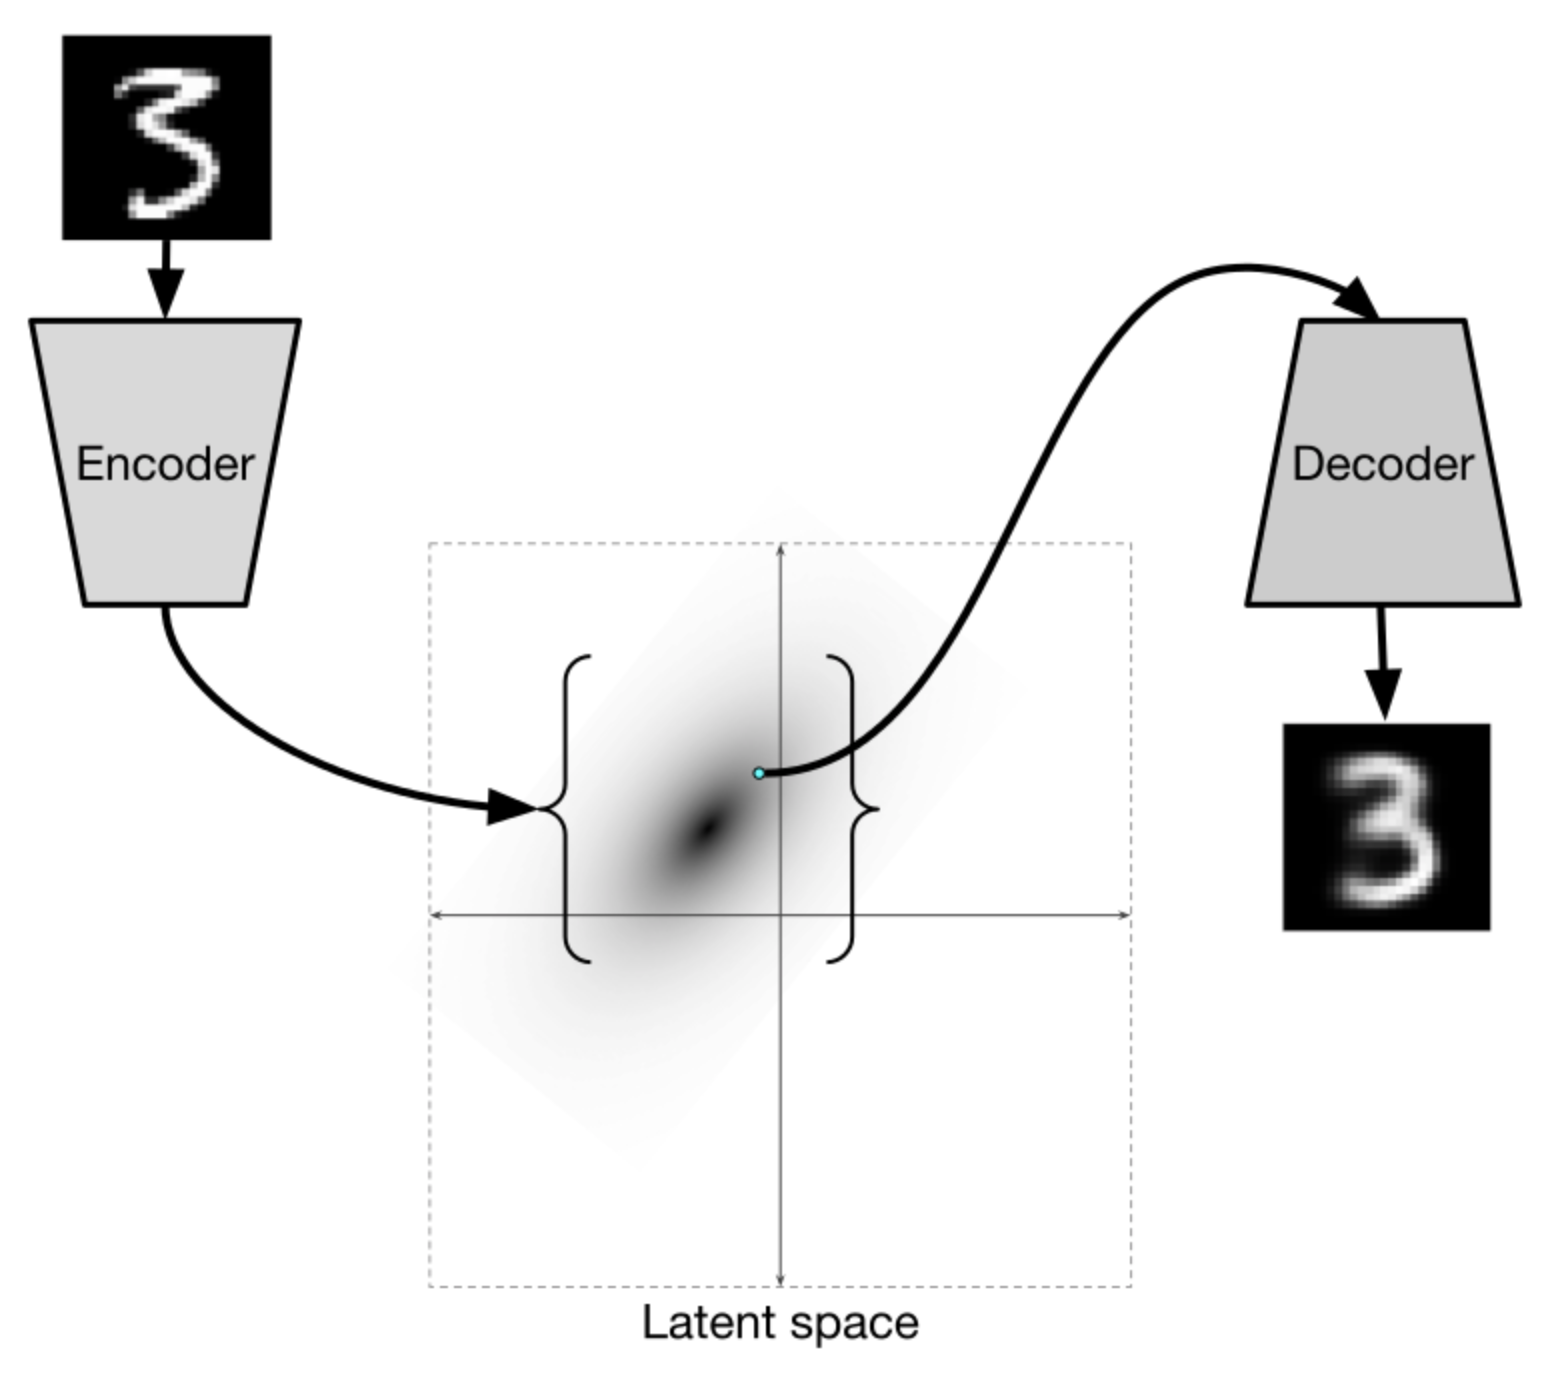
\includegraphics[width=\linewidth]{figs/VAE}
		\end{figure}
	\end{minipage}%
	\begin{minipage}[t]{0.4\columnwidth}
		\begin{figure}[h]
			\centering
			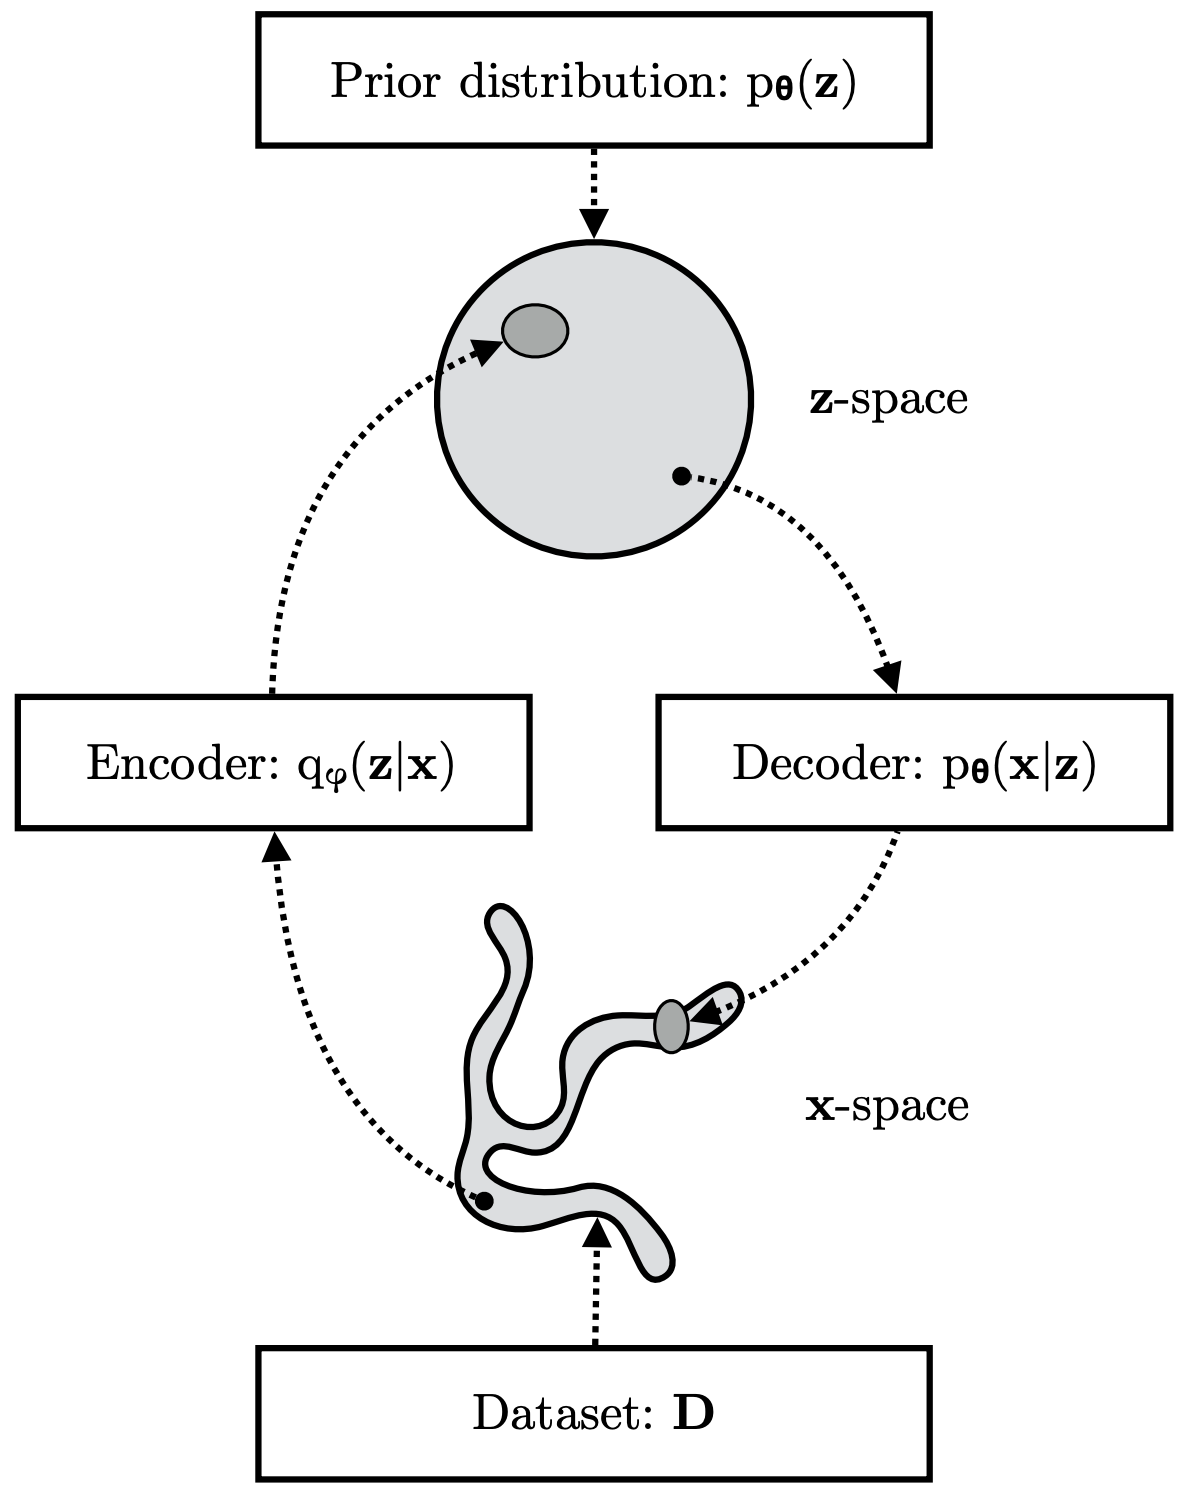
\includegraphics[width=\linewidth]{figs/vae_scheme}
		\end{figure}
	\end{minipage}
\end{frame}
%=======
\begin{frame}{Outline}
	\tableofcontents
\end{frame}
%=======
\section{ELBO Surgery}
%=======
\begin{frame}{ELBO Surgery}
	\myfootnotewithlink{http://approximateinference.org/accepted/HoffmanJohnson2016.pdf}{Hoffman M. D., Johnson M. J. ELBO Surgery: Yet Another Way to Carve Up the Variational Evidence Lower Bound, 2016}
	\vspace{-0.3cm}
	\[
	    \frac{1}{n} \sum_{i=1}^n \cL_{\bphi, \btheta}(\bx_i) = \frac{1}{n} \sum_{i=1}^n \Bigl[ \bbE_{q_{\bphi}(\bz| \bx_i)} \log \pt(\bx_i | \bz) - \KL(q_{\bphi}(\bz| \bx_i) \| p(\bz)) \Bigr].
	\]
    \eqpause
	\vspace{-0.3cm}
	\begin{block}{Theorem}
		\vspace{-0.5cm}
		\[
		    \frac{1}{n} \sum_{i=1}^n \KL(q_{\bphi}(\bz| \bx_i) \| p(\bz)) = {\color{violet} \KL(q_{\text{agg}, \bphi}(\bz) \| p(\bz))} + {\color{teal}\bbI_{q} [\bx, \bz]};
		\]
        \eqpause
		\vspace{-0.5cm}
		\begin{itemize}
			\item $q_{\text{agg}, \bphi}(\bz) = \frac{1}{n} \sum_{i=1}^n q_{\bphi}(\bz| \bx_i)$ denotes the \textbf{aggregated} variational posterior.
			\item $\bbI_{q} [\bx, \bz]$ is the mutual information between $\bx$ and $\bz$ under the data distribution $\pd(\bx)$ and $q_{\bphi}(\bz| \bx)$.
			\item  {\color{violet} The first term} encourages $q_{\text{agg}, \bphi}(\bz)$ to match the prior $p(\bz)$.
			\item {\color{teal} The second term} reduces the information about $\bx$ encoded in~$\bz$.
		\end{itemize}
	\end{block}
\end{frame}
%=======
\begin{frame}{ELBO Surgery}
	\myfootnotewithlink{http://approximateinference.org/accepted/HoffmanJohnson2016.pdf}{Hoffman M. D., Johnson M. J. ELBO Surgery: Yet Another Way to Carve Up the Variational Evidence Lower Bound, 2016}
		\vspace{-0.4cm}
		\[
		    \frac{1}{n} \sum_{i=1}^n \KL(q_{\bphi}(\bz| \bx_i) \| p(\bz)) = \KL(q_{\text{agg}, \bphi}(\bz) \| p(\bz)) + \bbI_q [\bx, \bz].
		\]
		\vspace{-0.3cm}
	\begin{block}{Proof}
		\vspace{-0.5cm}
		{\footnotesize
		\begin{multline*}
		    \frac{1}{n} \sum_{i=1}^n \KL(q_{\bphi}(\bz| \bx_i) \| p(\bz)) = \frac{1}{n} \sum_{i=1}^n \int q_{\bphi}(\bz| \bx_i) \log \frac{q_{\bphi}(\bz| \bx_i)}{p(\bz)} d \bz
		    \nextonslide{= \\= \frac{1}{n} \sum_{i=1}^n \int q_{\bphi}(\bz| \bx_i) \log \frac{{\color{violet}q_{\text{agg}, \bphi}(\bz)} {\color{teal}q_{\bphi}(\bz| \bx_i)}}{{\color{violet}p(\bz)} {\color{teal}q_{\text{agg}, \bphi}(\bz)}} d \bz}
		    \nextonslide{= \\ = \int \frac{1}{n} \sum_{i=1}^n  q_{\bphi}(\bz| \bx_i) \log {\color{violet}\frac{q_{\text{agg}, \bphi}(\bz)}{p(\bz)}} d \bz + \frac{1}{n}\sum_{i=1}^n \int q_{\bphi}(\bz| \bx_i) \log {\color{teal}\frac{q_{\bphi}(\bz| \bx_i)}{q_{\text{agg}, \bphi}(\bz)}} d \bz}
		    \nextonslide{= \\ = \KL (q_{\text{agg}, \bphi}(\bz) \| p(\bz)) + \frac{1}{n}\sum_{i=1}^n \KL(q_{\bphi}(\bz| \bx_i) \| q_{\text{agg}, \bphi}(\bz))}
		\end{multline*}
        \eqpause
		}
		\vspace{-0.4cm}
		\[
			\bbI_{q} [\bx, \bz] = \frac{1}{n}\sum_{i=1}^n \KL(q_{\bphi}(\bz| \bx_i) \| q_{\text{agg}, \bphi}(\bz)).
		\]
	\end{block}
\end{frame}
%=======
\begin{frame}{ELBO Surgery}
	\myfootnotewithlink{http://approximateinference.org/accepted/HoffmanJohnson2016.pdf}{Hoffman M. D., Johnson M. J. ELBO Surgery: Yet Another Way to Carve Up the Variational Evidence Lower Bound, 2016}
	\vspace{-0.3cm}
	\begin{block}{Revisiting the ELBO}
		\vspace{-0.7cm}
		{\small
		\begin{multline*}
		    \frac{1}{n}\sum_{i=1}^n \cL_{\bphi, \btheta}(\bx_i) = \frac{1}{n} \sum_{i=1}^n \left[ \bbE_{q_{\bphi}(\bz| \bx_i)} \log \pt(\bx_i | \bz) - \KL(q_{\bphi}(\bz| \bx_i) \| p(\bz)) \right]
		    \nextonslide{= \\ = \underbrace{\frac{1}{n} \sum_{i=1}^n \bbE_{q_{\bphi}(\bz| \bx_i)} \log \pt(\bx_i | \bz)}_{\text{Reconstruction Loss}} - \underbrace{\vphantom{ \sum_{i=1}^n} \bbI_q [\bx, \bz]}_{\text{Mutual Information}} - \underbrace{\vphantom{ \sum_{i=1}^n} \KL(q_{\text{agg}, \bphi}(\bz) \| {\color{teal}p(\bz)})}_{\text{Marginal KL}}}
		\end{multline*}
		}
		\vspace{-0.3cm}
	\end{block}
    \eqpause
	The prior distribution $p(\bz)$ only appears in the last term.
    \eqpause
	\begin{block}{Optimal VAE Prior}
		\vspace{-0.7cm}
		\[
	  		\KL(q_{\text{agg}, \bphi}(\bz) \| p(\bz)) = 0 \quad \Leftrightarrow \quad p (\bz) = q_{\text{agg}, \bphi}(\bz) = \frac{1}{n} \sum_{i=1}^n q_{\bphi}(\bz| \bx_i).
		\]
        \eqpause
		\vspace{-0.4cm} \\
		Hence, the optimal prior $p(\bz)$ is the aggregated variational posterior $q_{\text{agg}, \bphi}(\bz)$.
	\end{block}
\end{frame}
%=======
\begin{frame}{Marginal KL}
	\myfootnotewithlink{https://arxiv.org/abs/1505.05770}{Rezende D. J., Mohamed S. Variational Inference with Normalizing Flows, 2015} 
	\[
		\KL(q_{\text{agg}, \bphi}(\bz) \| p(\bz))
	\]
	\vspace{-0.5cm}
	\begin{itemize}
		\item $q_{\bphi}(\bz| \bx) = \cN(\bmu_{\bphi}(\bx), \bsigma^2_{\bphi}(\bx))$ is unimodal. 
		\item It is generally believed that the \textbf{mismatch between} $p(\bz)$  \textbf{and} $q_{\text{agg}, \bphi}(\bz)$  is the primary explanation for blurry VAE-generated images.
	\end{itemize}
    \eqpause
	\begin{figure}
		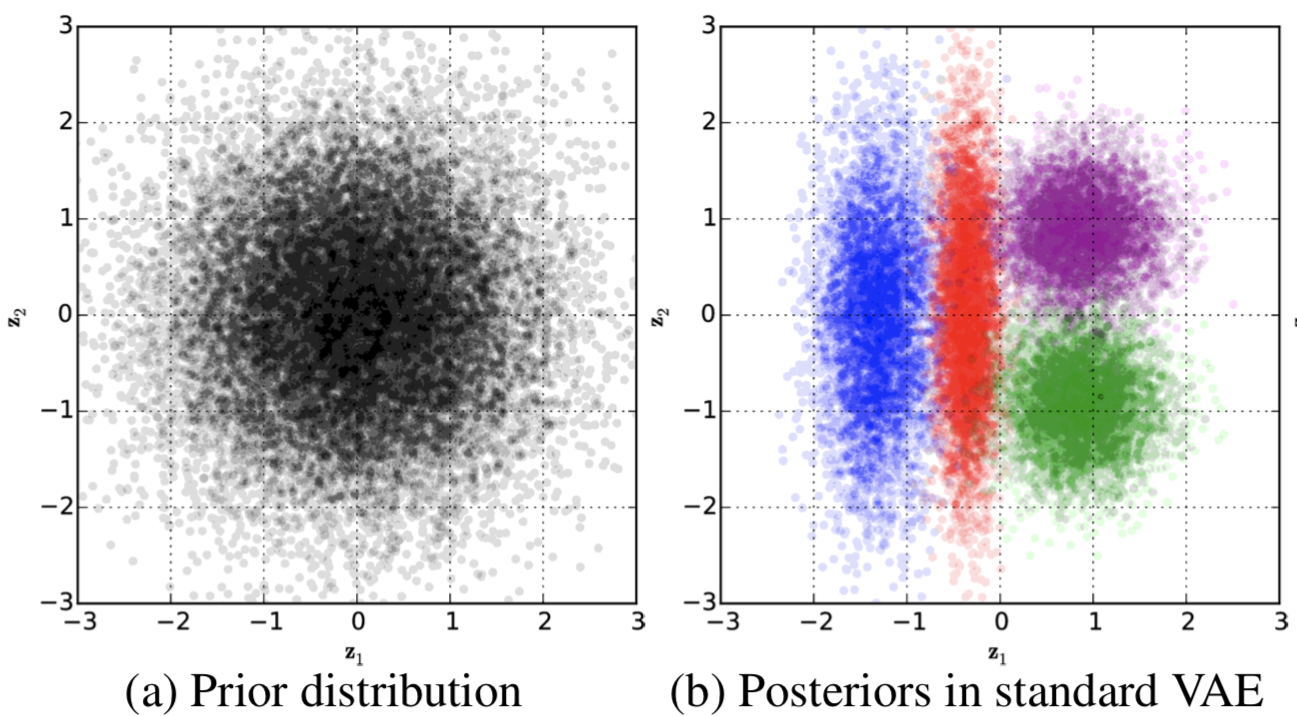
\includegraphics[width=0.8\linewidth]{figs/agg_posterior}
	\end{figure}
\end{frame}
%=======
\begin{frame}{Why are VAE Generations Blurry?}
	\myfootnotewithlink{https://arxiv.org/abs/2510.21890}{Lai C. H. et al. The principles of diffusion models, 2025.}
	
	Consider a Gaussian decoder $\pt(\bx | \bz) = \cN(\bmu_{\btheta}(\bz), \sigma^2 \bI)$.
	\eqpause
	\begin{block}{ELBO Optimization}
		With \textbf{fixed} encoder $q_{\bphi}(\bz | \bx)$, optimizing ELBO reduces to
		\vspace{-0.3cm}
		\[
			\argmin_{\btheta} \bbE_{\pd(\bx) q_{\bphi}(\bz | \bx)} \| \bx - \bmu_{\btheta}(\bz) \|^2
		\]
		The optimal decoder mean is the \textbf{conditional expectation}:
		\vspace{-0.3cm}
		\[
			\bmu^*(\bz) = \bbE_{q_{\bphi}(\bx | \bz)}[\bx] = \frac{\bbE_{\pd(\bx)}[q_{\bphi}(\bz | \bx) \cdot \bx]}{\bbE_{\pd(\bx)}[q_{\bphi}(\bz | \bx)]}
		\]
		\vspace{-0.7cm}
	\end{block}
	\eqpause
	\begin{block}{Blurriness from Averaging}
		\begin{itemize}
			\item $\pd(\bx)$ and $q_{\bphi}(\bz | \bx)$ give us the aggregated posterior $q_{\text{agg}, \bphi}(\bz)$.
			\item If $\bx \neq \bx'$ map to overlapping latent regions, $\bmu^*(\bz)$ averages over unrelated inputs.
			\item This leads to \textbf{blurry, non-distinct outputs}.
		\end{itemize}
	\end{block}
\end{frame}
%=======
\section{Discrete VAE Latent Representations}
%=======
\begin{frame}{Discrete VAE Latents}
	\begin{block}{Motivation}
		\begin{itemize}
			\item VAE has used \textbf{continuous} latent variables $\bz$.
			\item For some modalities, \textbf{discrete} representations $\bz$ may be a more natural choice.
			\item Advanced autoregressive models are highly effective for distributions over discrete variables (for example, transformers process discrete tokens).
		\end{itemize}
	\end{block}
	\eqpause
	\begin{block}{ELBO}
		\vspace{-0.3cm}
		\[
			\cL_{\bphi, \btheta}(\bx)  = \bbE_{q_{\bphi}(\bz| \bx)} \log \pt(\bx| \bz) - \KL(q_{\bphi}(\bz| \bx) \| p(\bz)) \rightarrow \max_{\bphi, \btheta}.
		\]
		\vspace{-0.5cm}
	\end{block}
	\eqpause
	\begin{itemize}
		\item Apply the reparametrization trick to obtain unbiased gradients.
		\item Use Gaussian distributions for $q_{\bphi}(\bz| \bx)$ and $p(\bz)$ to compute the KL analytically.
	\end{itemize}
\end{frame}
%=======
\begin{frame}{Discrete VAE Latents}
	\begin{block}{Assumptions}
		\begin{itemize}
			\item Let $c \sim \Cat(\bpi)$, where 
			\vspace{-0.6cm}
			\[
			\bpi = (\pi_1, \dots, \pi_K), \quad \pi_k = P(c = k), \quad \sum_{k=1}^K \pi_k = 1.
			\]
			\vspace{-0.6cm}
			\item Suppose the VAE adopts a discrete latent variable $c$ with prior $p(c) = \Uniform\{1, \dots, K\}$.
		\end{itemize}
	\end{block}
	\eqpause
	\begin{block}{ELBO}
		\vspace{-0.5cm}
		\[
			\cL_{\bphi, \btheta}(\bx)  = \bbE_{q_{\bphi}(c| \bx)} \log \pt(\bx| c) - {\color{olive} \KL(q_{\bphi}(c| \bx) \| p(c))} \rightarrow \max_{\bphi, \btheta}.
		\]
	\end{block}
	\vspace{-1.0cm}
	{\small
	\begin{multline*}
		{\color{olive} \KL(q_{\bphi}(c| \bx) \| p(c))} = \sum_{k=1}^K q_{\bphi}(k| \bx) \log \frac{q_{\bphi}(k| \bx)}{p(k)} 
		\nextonslide{= \\ = \color{violet}{\sum_{k=1}^K q_{\bphi}(k| \bx) \log q_{\bphi}(k| \bx)}  \color{teal}{- \sum_{k=1}^K q_{\bphi}(k| \bx) \log p(k)}}
		\nextonslide{= \\ = \color{violet}{- \Ent(q_{\bphi}(c| \bx))} + \color{teal}{\log K}. }
	\end{multline*}
	}
\end{frame}
%=======
\begin{frame}{Discrete VAE Latents}
	\myfootnotewithlink{https://arxiv.org/abs/2403.18103}{Chan S., Tutorial on Diffusion Models for Imaging and Vision, 2024}
	\[
		\cL_{\bphi, \btheta}(\bx)  = \bbE_{q_{\bphi}(c| \bx)} \log \pt(\bx| c) + \Ent(q_{\bphi}(c| \bx)) - \log K \rightarrow \max_{\bphi, \btheta}.
	\]
	\eqpause
	\vspace{-0.5cm}
	\begin{itemize}
		\item The encoder should output a discrete distribution $q_{\bphi}(c| \bx)$.
					\item We need an analogue of the reparametrization trick for discrete $q_{\bphi}(c| \bx)$.
		\item The decoder $\pt(\bx| c)$ must take a discrete random variable $c$ as input.
	\end{itemize}
	\begin{figure}[h]
		\centering
		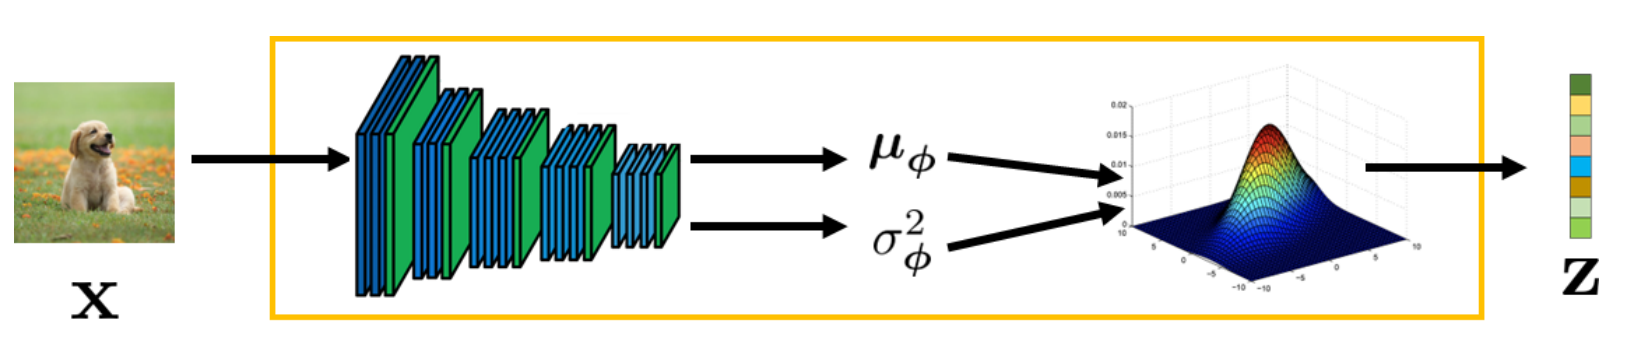
\includegraphics[width=0.7\linewidth]{figs/vae-encoder}
	\end{figure}
	\begin{figure}[h]
		\centering
		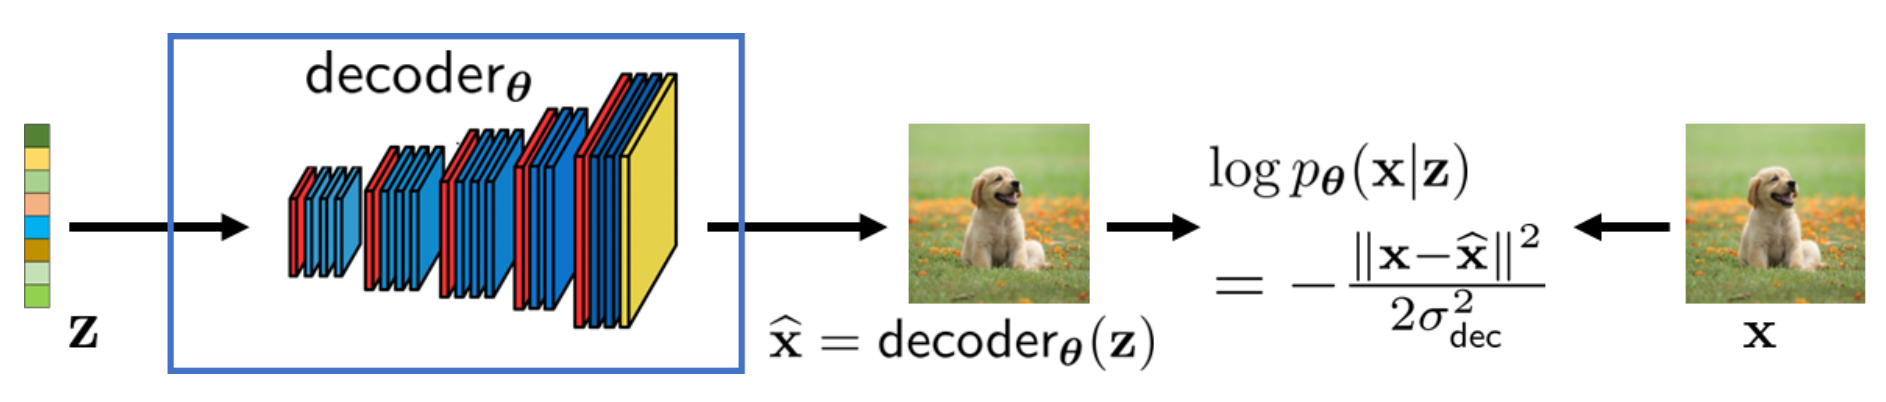
\includegraphics[width=0.9\linewidth]{figs/vae-decoder}
	\end{figure}
\end{frame}
%=======
\section{Vector Quantized VAE}
%=======
\begin{frame}{Vector Quantization}
	\myfootnotewithlink{https://arxiv.org/abs/2004.02088}{Zhao Y. et al. Feature Quantization Improves GAN Training, 2020} 
	Define the codebook (dictionary) space $\{\be_k\}_{k=1}^K$ with $\be_k \in \bbR^L$ and $K$ the number of codebook entries.
    \eqpause
	\begin{block}{Quantized Representation}
		A quantized vector $\bz_q \in \bbR^{L}$, for any $\bz \in \bbR^L$, is defined via nearest-neighbor lookup in the codebook:
		\vspace{-0.3cm}
		\[
			\bz_q = \bq (\bz) = \be_{k^*}, \quad \text{where } k^* = \argmin_k \| \bz - \be_k \|.
		\] 
		\vspace{-0.7cm}
	\end{block}
	\eqpause
	\vspace{-0.2cm}
	\begin{block}{Quantization Procedure}
		If the encoded tensor has spatial dimensions, quantization is independently applied to each of the $W \times H$ locations.
		\begin{minipage}[t]{0.65\columnwidth}
			\begin{figure}
				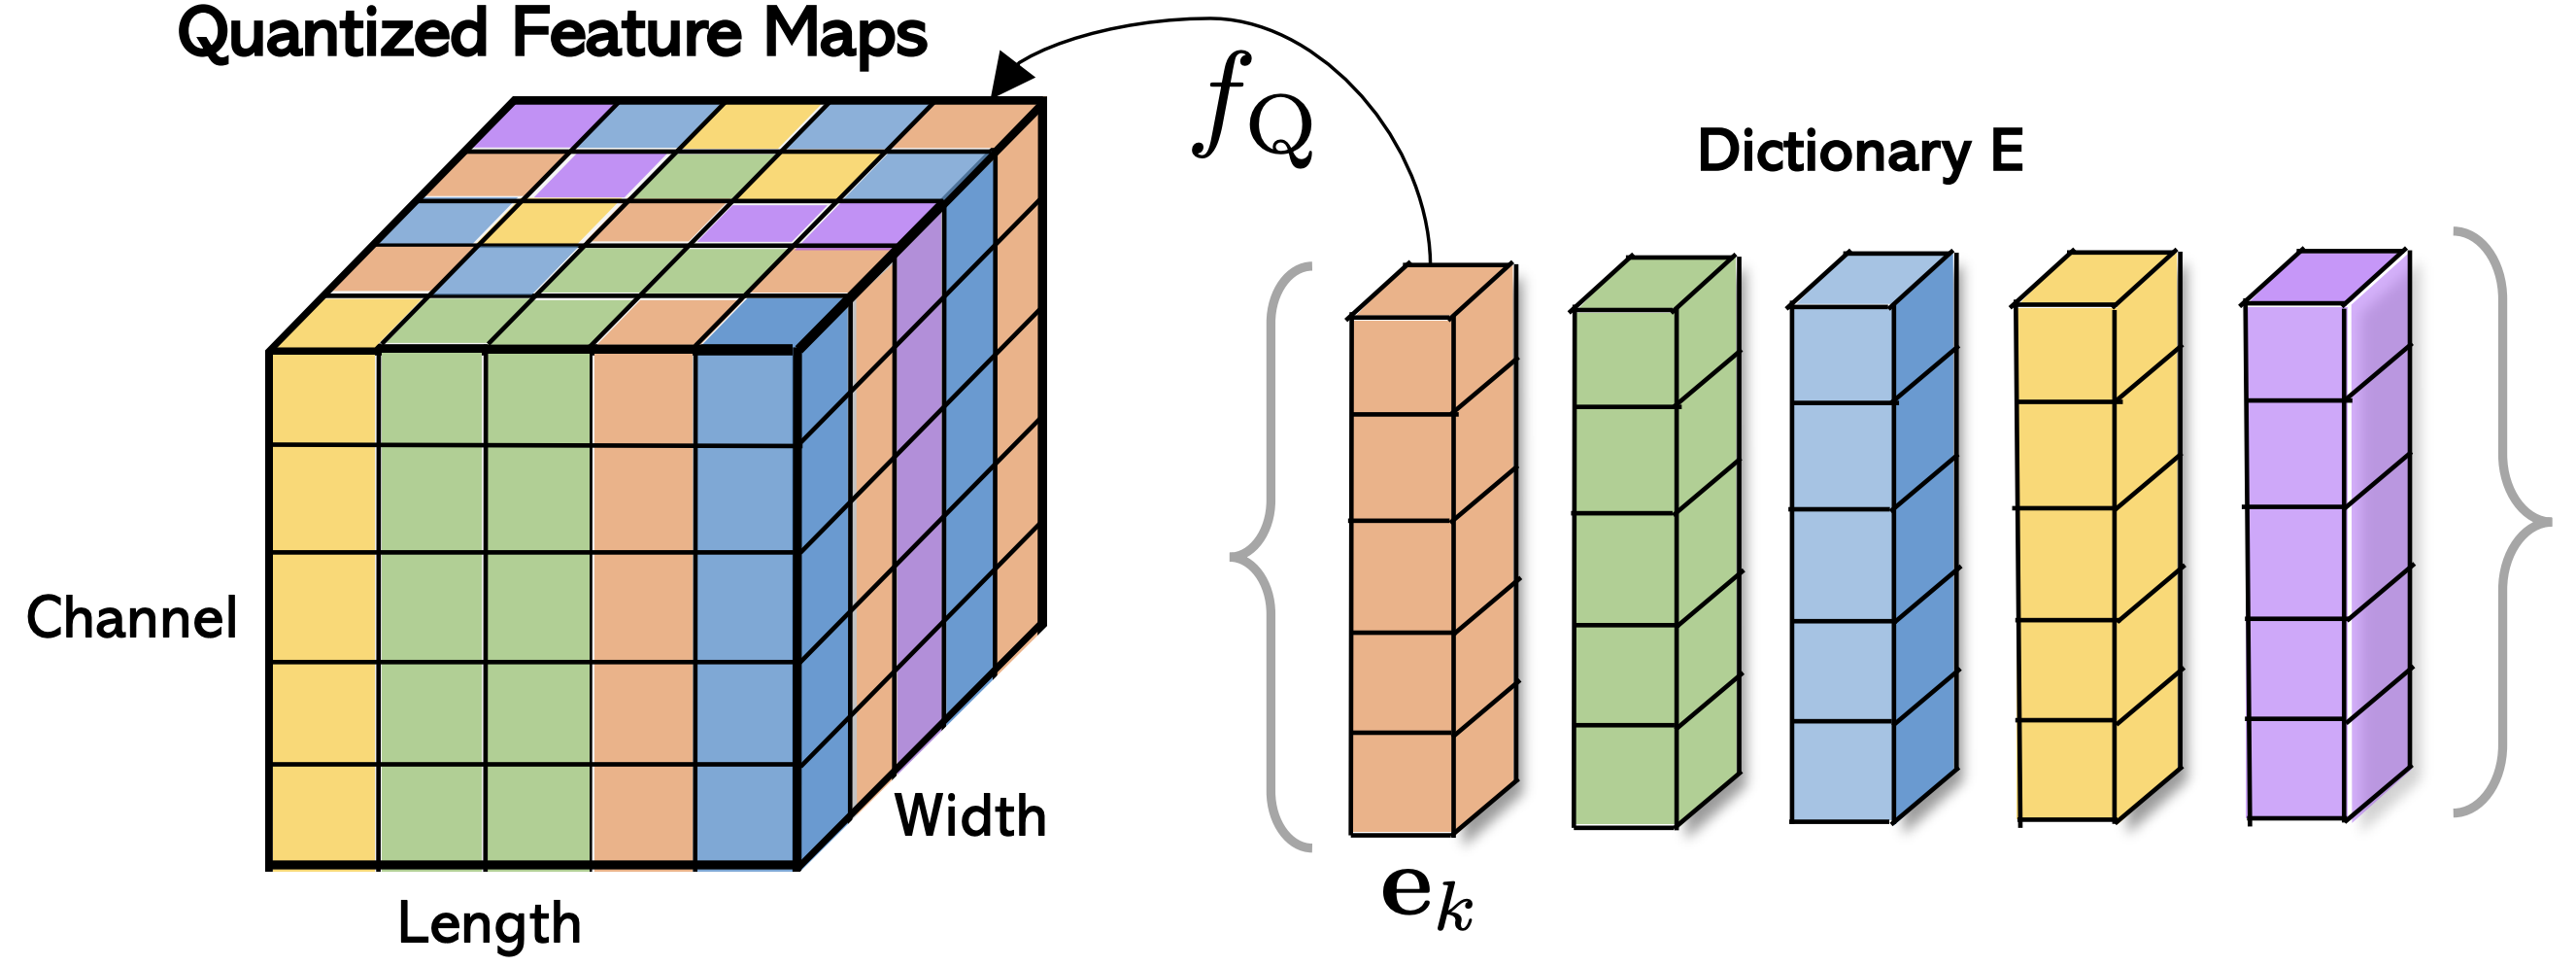
\includegraphics[width=0.8\linewidth]{figs/fqgan_cnn.png}
			\end{figure}
		\end{minipage}%
		\begin{minipage}[t]{0.35\columnwidth}
			\begin{figure}
				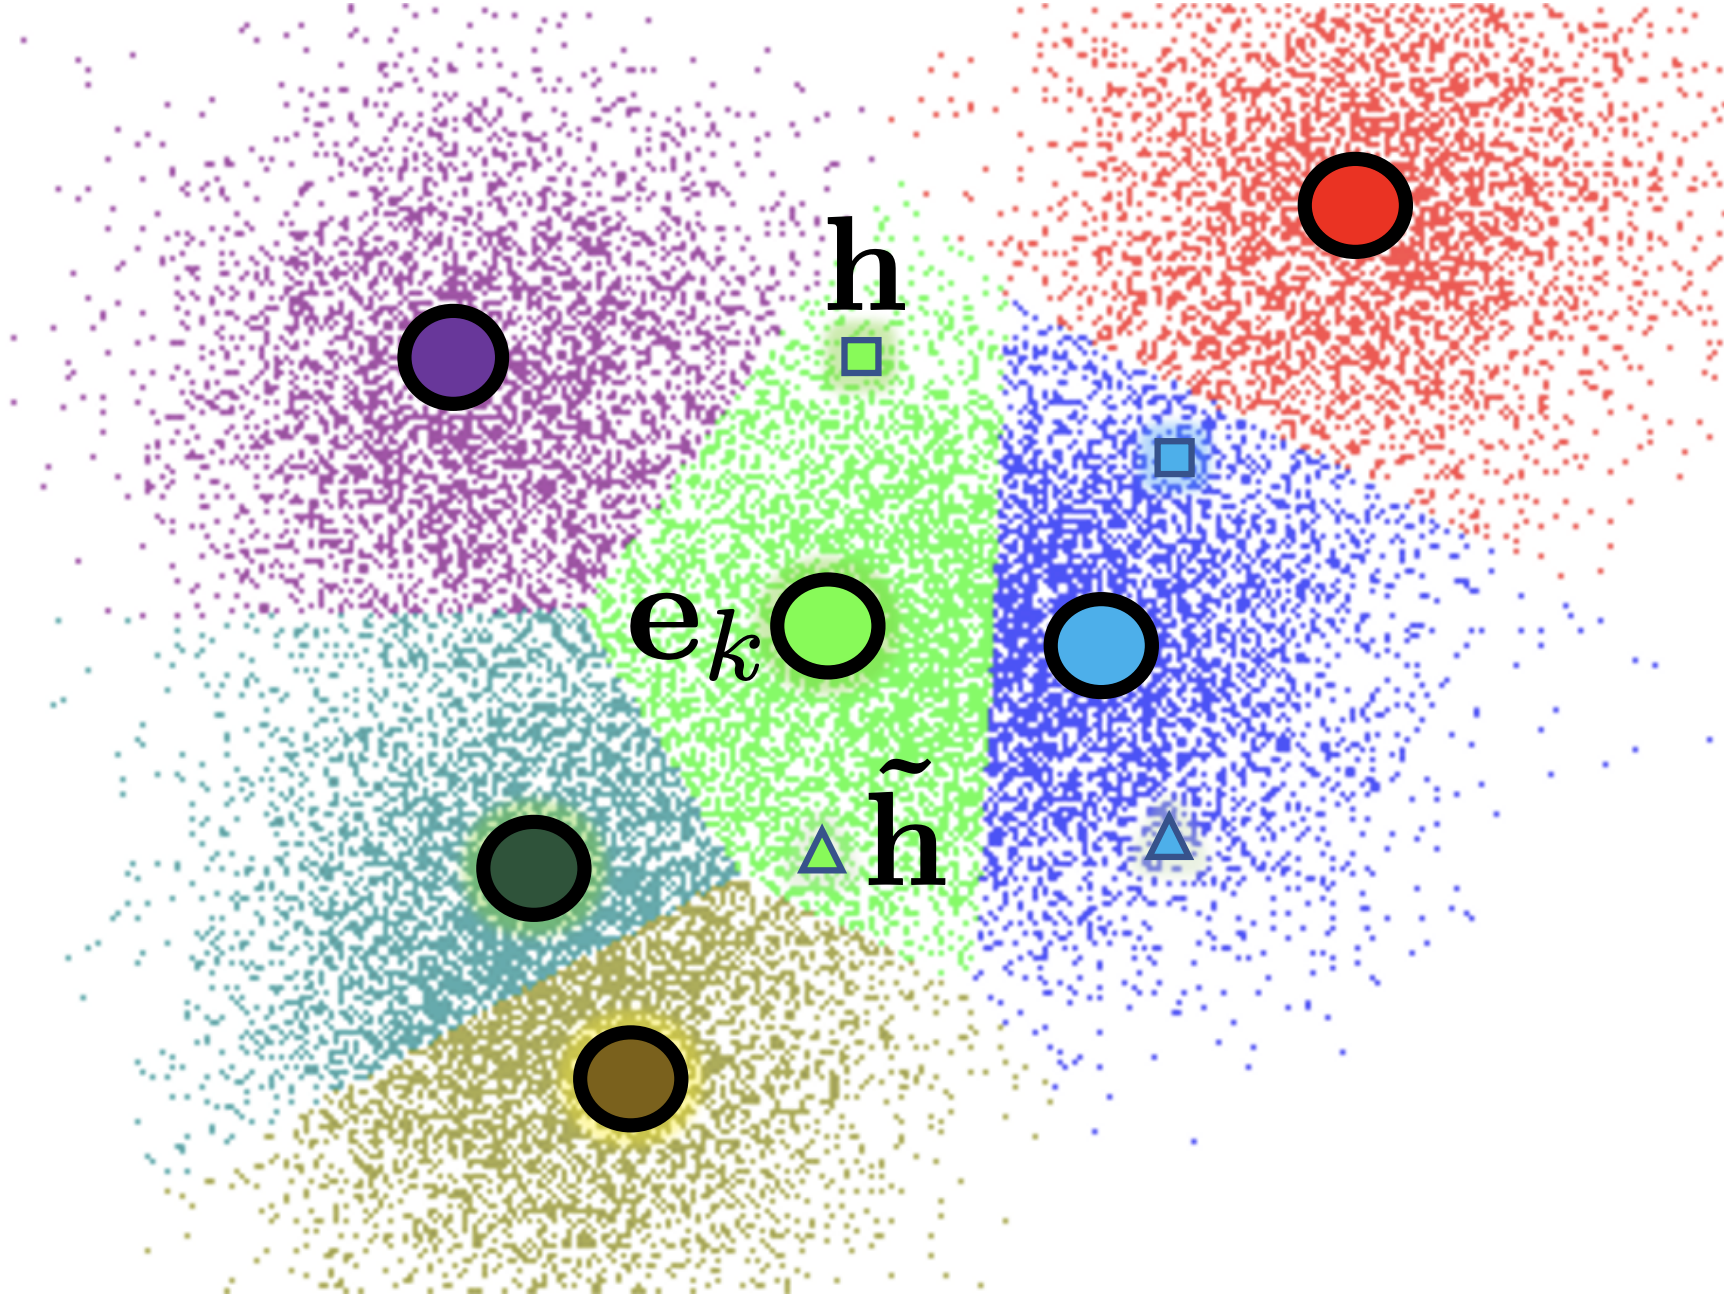
\includegraphics[width=0.7\linewidth]{figs/fqgan_lookup}
			\end{figure}
		\end{minipage}
	\end{block}
\end{frame}
%=======
\begin{frame}{Vector Quantized VAE (VQ-VAE)}
	\myfootnotewithlink{https://arxiv.org/abs/1711.00937}{Oord A., Vinyals O., Kavukcuoglu K. Neural Discrete Representation Learning, 2017} 
	\begin{itemize}
		\item The encoder outputs a continuous vector $\bz_e = \NN_{e, \bphi}(\bx) \in \bbR^{L}$.
		\item Quantization deterministically maps $\bz_e$ to its quantized codebook vector $\bz_q$.
		\item The decoder is conditioned on codebook entries $\be_c$, i.e., via $\pt(\bx | \be_c)$ (instead of $\pt(\bx| c)$).
	\end{itemize}
    \eqpause
	\begin{block}{Deterministic Variational Posterior}
		\vspace{-0.3cm}
		\[
			q_{\bphi}(c = k^* | \bx) = \begin{cases}
				1 , \quad \text{for } k^* = \argmin_k \| \bz_e - \be_k \|; \\
				0, \quad \text{otherwise}.
		\end{cases}
		\]
        \eqpause
		\[
			\KL(q_{\bphi}(c| \bx) \| p(c)) = - \underbrace{\Ent(q_{\bphi}(c| \bx))}_{=0} + \log K = \log K. 
		\]
        \eqpause
	\end{block}	
	\vspace{-0.4cm}
	\textbf{Note:} The KL regularizer becomes constant and has no direct effect on the ELBO objective in this case.
\end{frame}
%=======
\begin{frame}{Vector Quantized VAE (VQ-VAE): Forward}
	\myfootnotewithlink{https://arxiv.org/abs/1711.00937}{Oord A., Vinyals O., Kavukcuoglu K. Neural Discrete Representation Learning, 2017} 
	\begin{block}{Deterministic Variational Posterior}
		\vspace{-0.3cm}
		\[
			q_{\bphi}(c = k^* | \bx) = \begin{cases}
			1 , \quad \text{for } k^* = \argmin_k \| \bz_e - \be_k \|; \\
			0, \quad \text{otherwise}.
			\end{cases}
		\]
	\vspace{-0.5cm}
	\end{block}	
    \eqpause
	\begin{block}{ELBO}
		\vspace{-0.6cm}
		\[
			\cL_{\bphi, \btheta}(\bx)  = \bbE_{q_{\bphi}(c| \bx)} \log \pt(\bx| \be_{c}) - \log K \nextonslide{= \log \pt(\bx| \bz_q) - \log K,}
		\]
		where $\bz_q = \be_{k^*}$, $k^* = \argmin_k \| \bz_e - \be_k \|$.
	\end{block}
    \eqpause
	\vspace{-0.3cm} 
	\begin{figure}
		\centering
		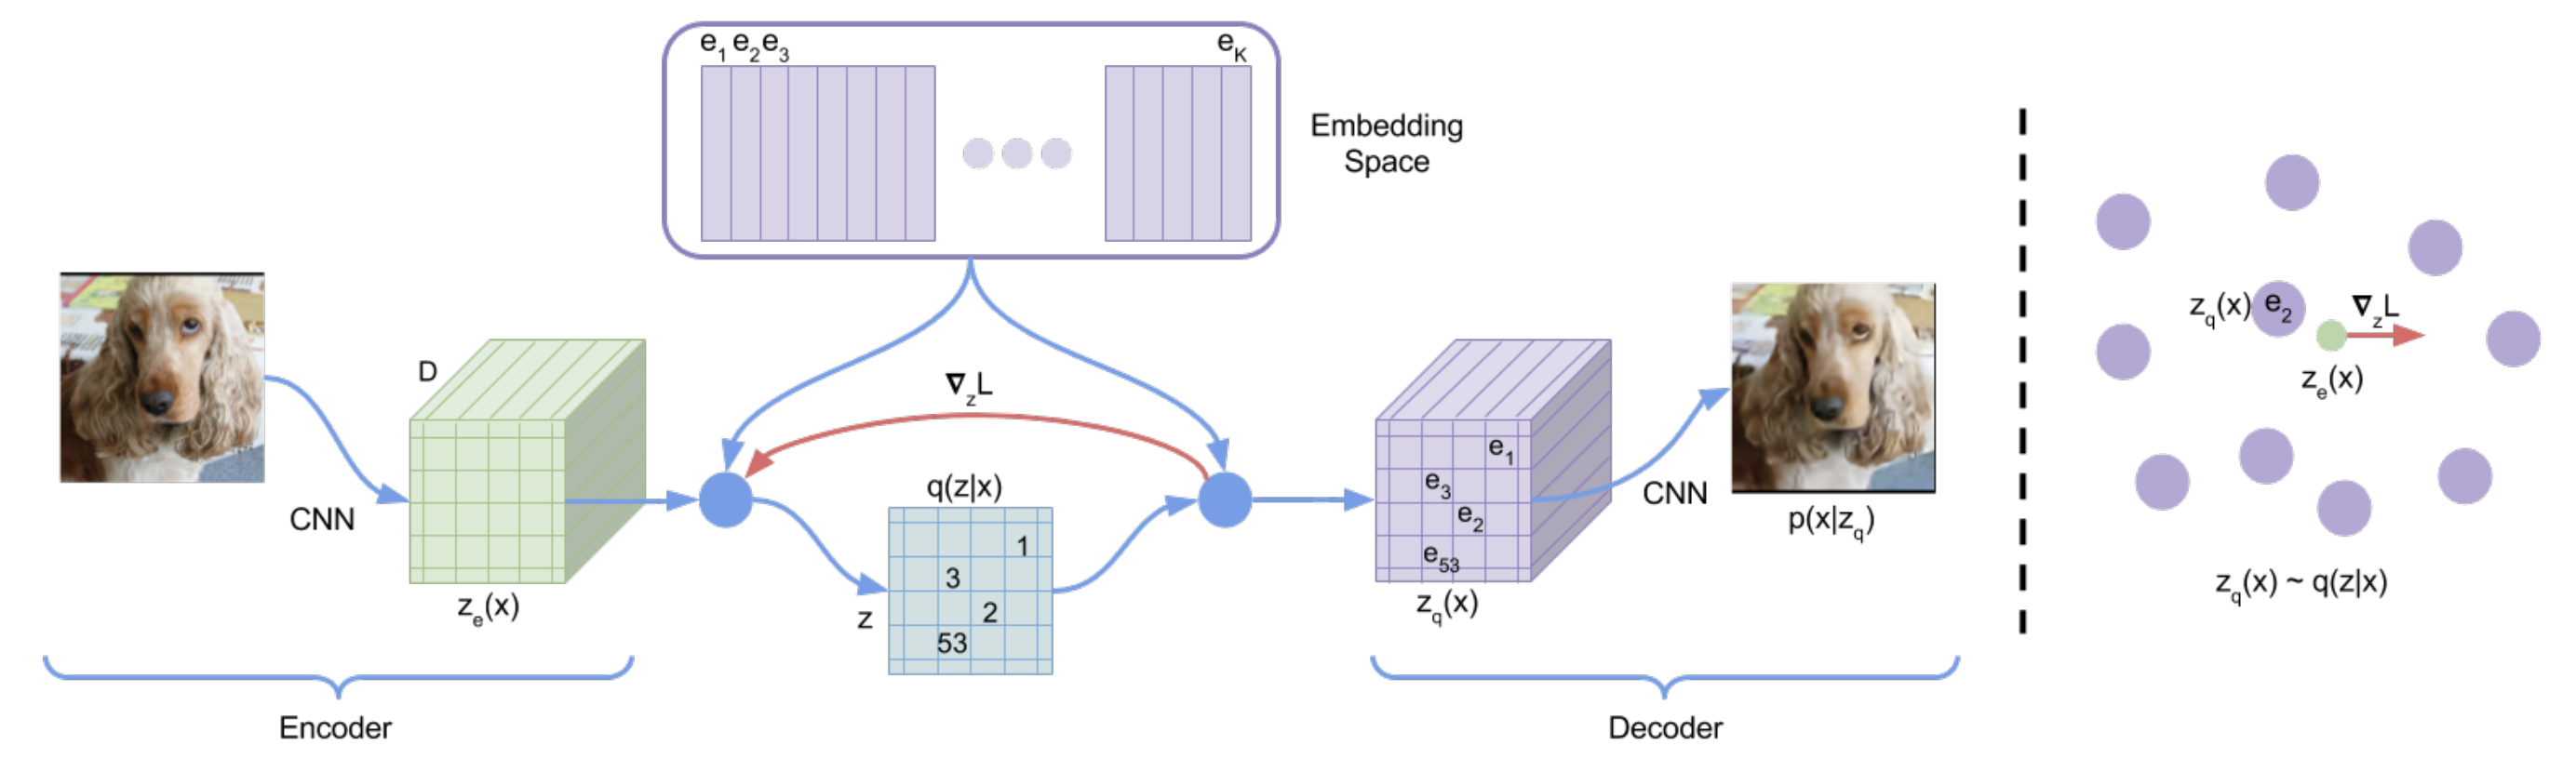
\includegraphics[width=0.85\linewidth]{figs/vqvae}
	\end{figure}
    \eqpause
	\vspace{-0.3cm} 
	\textbf{Challenge:} The $\argmin$ operation is non-differentiable.
\end{frame}
%=======
\begin{frame}{Vector Quantized VAE (VQ-VAE): Backward}
	\myfootnotewithlink{https://arxiv.org/abs/1711.00937}{Oord A., Vinyals O., Kavukcuoglu K. Neural Discrete Representation Learning, 2017} 
	\begin{block}{ELBO}
		\vspace{-0.5cm}
		\[
			\cL_{\bphi, \btheta}(\bx)  =  \log \pt(\bx| \bz_q) - \log K, \quad \bz_q = \be_{k^*},\; k^* = \argmin_k \| \bz_e - \be_k \|.
		\]
		\vspace{-0.5cm}
	\end{block}
    \eqpause
	\begin{figure}
		\centering
		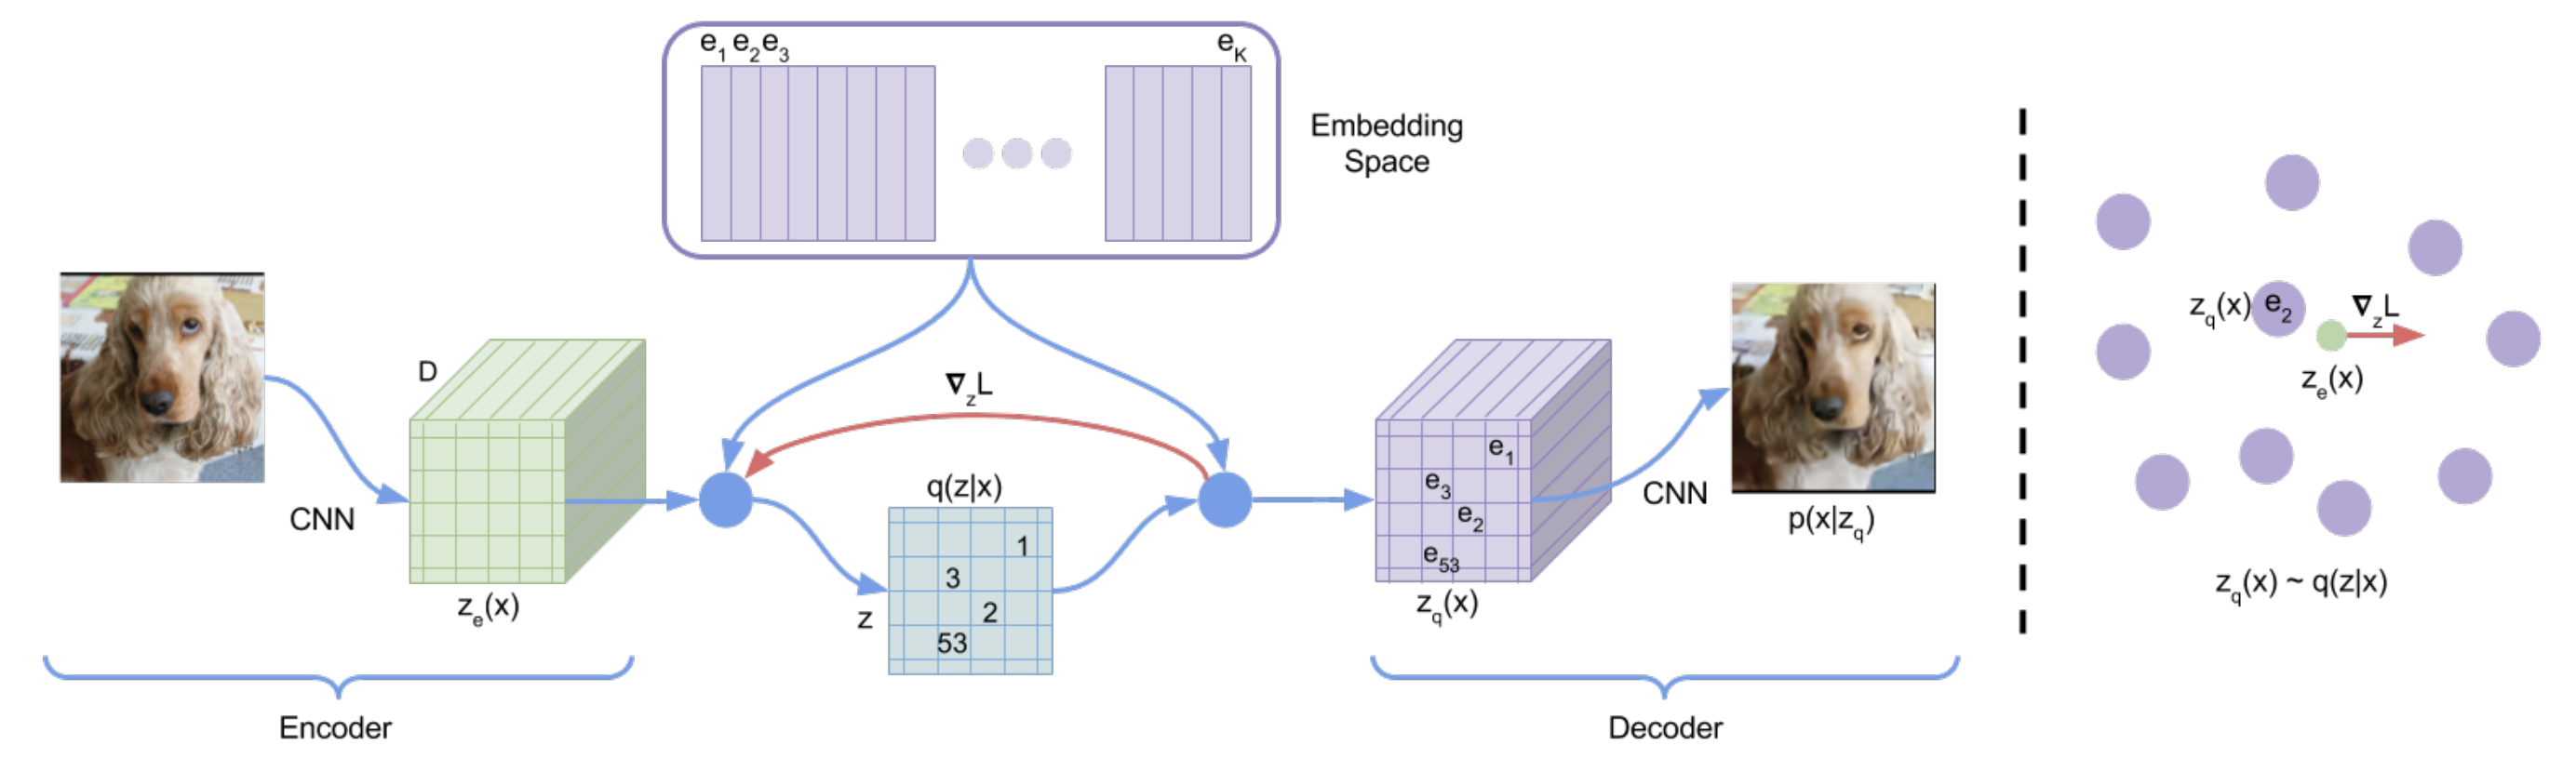
\includegraphics[width=0.85\linewidth]{figs/vqvae}
	\end{figure}
    \eqpause
	\vspace{-0.3cm}
	\begin{block}{Straight-Through Gradient Estimator}
		\vspace{-0.5cm}
		\begin{multline*}
		\frac{\partial \log p(\bx | \bz_q , \btheta)}{\partial \bphi} = \frac{\partial \log \pt(\bx| \bz_q)}{\partial \bz_q} \cdot {\color{red}\frac{\partial \bz_q}{\partial \bphi}} = \\
		\nextonslide{= \frac{\partial \log \pt(\bx| \bz_q)}{\partial \bz_q} \cdot {\color{red}\frac{\partial \bz_q}{\partial \bz_e}} \cdot \frac{\partial \bz_e}{\partial \bphi}}
		\nextonslide{\approx \frac{\partial \log \pt(\bx| \bz_q)}{\partial \bz_q} \cdot \frac{\partial \bz_e}{\partial \bphi}}
		\end{multline*}
	\end{block}
\end{frame}
%=======
\begin{frame}{Vector Quantized VAE-2 (VQ-VAE-2)}
	\myfootnotewithlink{https://arxiv.org/abs/1906.00446}{Razavi A., Oord A., Vinyals O. Generating Diverse High-Fidelity Images with VQ-VAE-2, 2019} 
	Extension to the spatial domain: $\bc \in \{1, \dots, K\}^{W \times H}$
	\vspace{-0.3cm}
	\[
		q_{\bphi}(\bc | \bx) = \prod_{i=1}^W \prod_{j=1}^H q(c_{ij} | \bx, \bphi); \quad p(\bc) = \prod_{i=1}^W \prod_{j=1}^H \Uniform\{1, \dots, K\}.
	\]
	\vspace{-0.6cm}
	\begin{block}{Sample Diversity}
		\vspace{-0.2cm}
		\begin{figure}
			\centering
			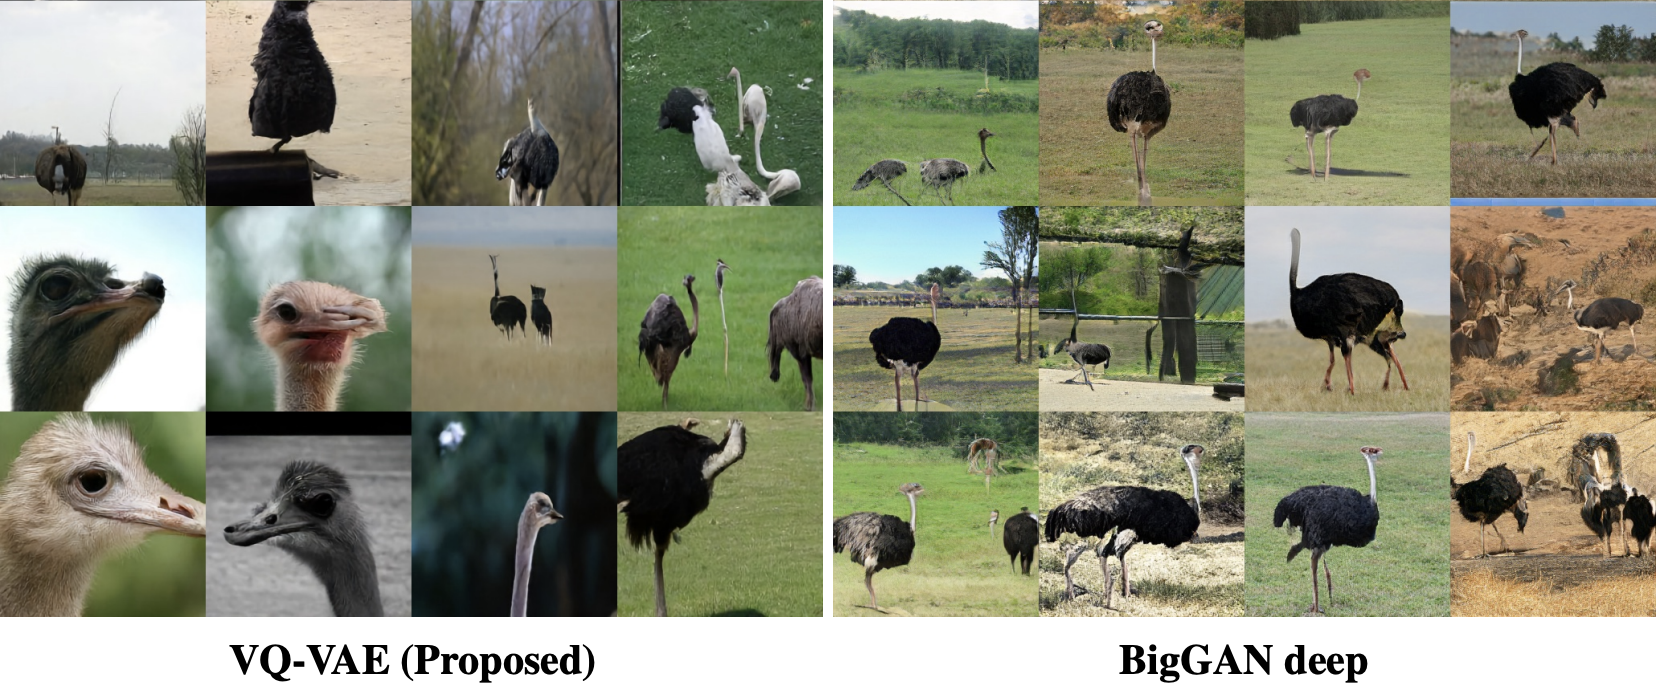
\includegraphics[width=1.0\linewidth]{figs/vqvae2_diversity}
		\end{figure}
	\end{block}
\end{frame}
%=======
\begin{frame}{Vector Quantized VAE (VQ-VAE): Final algorithm}
	\begin{block}{Training}
		\begin{itemize}
			\item Vector-quantize (per spatial location if applicable):
			\vspace{-0.3cm}
			\[
				k^* = \argmin_k \|\bz_e - \be_k\|_2, \quad \bz_q = \be_{k^*}, \quad \bz_e = \NN_{e,\bphi}(\bx).
			\]
			\vspace{-0.5cm}
			\item Compute ELBO objective:
			\vspace{-0.3cm}
			\[
				\cL_{\bphi, \btheta}(\bx) = \log \pt(\bx | \bz_q) - \log K.
			\]
			\vspace{-0.5cm}
			\item Compute total loss with codebook and commitment losses (with stop-gradient $\text{sg}[\cdot]$):
			\vspace{-0.3cm}
			\[
				\cL = - \cL_{\bphi, \btheta}(\bx) + \big\|\text{sg}[\bz_e] - \be_{k^*}\big\|_2^2 + \beta \big\|\bz_e - \text{sg}[\be_{k^*}]\big\|_2^2
			\]
			\vspace{-0.5cm}
			\item Use straight-through gradient estimation for encoder.
		\end{itemize}
	\end{block}
	\eqpause
	\vspace{-0.3cm}
	\begin{block}{Sampling}
		\begin{itemize}
			\item Sample $c \sim p(c) = \Uniform\{1, \dots, K\}$.
			\item Generate $\bx \sim \pt(\bx | \be_c)$.
		\end{itemize}
	\end{block}
\end{frame}
%=======
\section{Likelihood-Free Learning}
%=======
\begin{frame}{Likelihood-Based Models}
	\myfootnotewithlink{https://arxiv.org/abs/1511.01844}{Theis L., Oord A., Bethge M. A Note on the Evaluation of Generative Models, 2015}
	\begin{minipage}[t]{0.48\columnwidth}
		\vspace{-0.3cm}
		\begin{block}{Poor Likelihood \\ High-Quality Samples}
			\vspace{-0.3cm}
			\[
				p_1(\bx) = \frac{1}{n} \sum_{i=1}^n \cN(\bx | \bx_i, \epsilon \bI)
			\]
			If $\epsilon$ is very small, this model produces excellent, sharp samples but achieves poor likelihoods on test data.
		\end{block}	
	\end{minipage}%
	\begin{minipage}[t]{0.52\columnwidth}
		\eqpause
		\vspace{-0.3cm}
		\begin{block}{High Likelihood \\ Poor Samples}
			\vspace{-0.5cm}
			\[
				p_2(\bx) = 0.01p(\bx) + 0.99p_{\text{noise}}(\bx)
			\]
			\vspace{-1.0cm}
			\begin{multline*}
				\log \left[ 0.01p(\bx) + 0.99p_{\text{noise}}(\bx) \right] \geq \\ \geq \log \left[ 0.01p(\bx) \right]  = \log p(\bx) - \log 100
			\end{multline*}
			This model contains mostly noisy, irrelevant samples; for high dimensions, $\log p(\bx)$ scales linearly with $m$.
		\end{block}
	\end{minipage}
	\eqpause
	\begin{itemize}
		\item Likelihood isn't always a suitable metric for evaluating generative models.
		\item Sometimes, the likelihood function can't even be computed exactly.
	\end{itemize}
\end{frame}
%=======
\begin{frame}{Likelihood-Free Learning}
	\begin{block}{Motivation}
	 We're interested in approximating the true data distribution~$\pd(\bx)$.
	Instead of searching over all distributions, let's learn a model $\pt(\bx) \approx \pd(\bx)$.
	\end{block}
	\eqpause
	Suppose we have two sets of samples: 
	\begin{itemize}
		\item $\{\bx_i\}_{i=1}^{n_1} \sim \pd(\bx)$ — real data;
		\item $\{\bx_i\}_{i=1}^{n_2} \sim \pt(\bx)$ — generated (fake) data.
	\end{itemize}
	\eqpause
	Define a discriminative model (classifier):
	\[
		p(y = 1 | \bx) = P(\bx \sim \pd(\bx)); \quad p(y = 0 | \bx) = P(\bx \sim \pt(\bx))
	\]
	\eqpause
	\vspace{-0.5cm}
	\begin{block}{Assumption}
		The generative model $\pt(\bx)$ matches $\pd(\bx)$ if a discriminative model $p(y | \bx)$ can't distinguish between them --- that is, if $p(y = 1 | \bx) = 0.5$ for every $\bx$.
	\end{block}
\end{frame}
%=======
\begin{frame}{Generative Adversarial Networks (GAN)}
	\myfootnotewithlink{https://arxiv.org/abs/1406.2661}{Goodfellow I. J. et al. Generative Adversarial Networks, 2014}
	\begin{itemize}
		\item The more expressive the discriminator, the closer we get to the optimal $\pt(\bx)$.
		\item Standard classifiers are trained by minimizing cross-entropy loss $-\bbE_{\hat{p}(\bx, y)} \log p(y | \bx)$ with $\hat{p}(\bx, y) = \frac{1}{2} \bbI_{y=1}\pd(\bx) + \frac{1}{2} \bbI_{y=0}\pt(\bx)$.
	\end{itemize}
	\eqpause
	\begin{block}{Cross-Entropy for Discriminator}
		\vspace{-0.3cm}
		\[
			\min_{p(y | \bx)} \left[ - \bbE_{\pd(\bx)} \log p(y = 1 | \bx) - \bbE_{\pt(\bx)} \log p(y = 0 | \bx) \right] 
		\]
		\[
			\max_{p(y | \bx)} \left[\bbE_{\pd(\bx)} \log p(y = 1 | \bx) + \bbE_{\pt(\bx)} \log p(y = 0 | \bx) \right] 
		\]
	\end{block}
	\eqpause
	\vspace{-0.3cm}
	\begin{block}{Generative Model}
		Suppose $\pt(\bx, \bz) = \pt(\bx| \bz) p(\bz)$, where $p(\bz)$ is a base distribution, and $\pt(\bx | \bz) = \delta (\bx - \bG_{\btheta}(\bz))$ is deterministic.
	\end{block}
\end{frame}
%=======
\begin{frame}{Generative Adversarial Networks (GAN)}
	\myfootnotewithlink{https://arxiv.org/abs/1406.2661}{Goodfellow I. J. et al. Generative Adversarial Networks, 2014}
	\begin{block}{Cross-Entropy for Discriminative Model}
		\vspace{-0.3cm}
		\[
			\max_{p(y | \bx)} \left[\bbE_{\pd(\bx)} \log p(y = 1 | \bx) + \bbE_{\pt(\bx)} \log p(y = 0 | \bx) \right] 
		\]
	\end{block}
	\eqpause
	\begin{itemize}
		\item \textbf{Discriminator:} A classifier $p_{\bphi}(y = 1 | \bx) = D_{\bphi}(\bx) \in [0, 1]$, distinguishing real and generated samples. The discriminator aims to \textbf{maximize} cross-entropy.
		\item \textbf{Generator:} The generative model $\bx = \bG_{\btheta}(\bz),\; \bz \sim p(\bz)$, seeks to fool the discriminator. The generator aims to \textbf{minimize} cross-entropy.
	\end{itemize}
	\eqpause
	\begin{block}{GAN Objective}
		\vspace{-0.5cm}
		\[
			\min_{G} \max_D \left[ \bbE_{\pd(\bx)} \log D(\bx) + \bbE_{\pt(\bx)} \log (1 - D(\bx)) \right] 
		\]
		\eqpause
		\[
			\min_{G} \max_D \left[ \bbE_{\pd(\bx)} \log D(\bx) + \bbE_{p(\bz)} \log (1 - D(\bG(\bz))) \right]
		\]
	\end{block}
\end{frame}
%=======
\begin{frame}{Summary}
	\begin{itemize}
		\item ELBO surgery gives insights into the prior's influence in VAEs; the optimal prior is the aggregated variational posterior. 
		\vfill
		\item The mismatch between $p(\bz)$ and $q_{\text{agg}, \bphi}(\bz)$ is widely regarded as the principal reason for VAE-generated image blurriness.		
		\vfill
		\item Vector quantization provides a way to construct VAEs with discrete latents and deterministic variational posteriors.
		\vfill
		\item The straight-through gradient estimator allows gradients to pass as if quantization were an identity operation during backpropagation.			
		\vfill
		\item Likelihood is not always a suitable metric for evaluating generative models
		\vfill
		\item Likelihood-free learning motivates the use of discriminative models to match distributions.
	\end{itemize}
\end{frame}
%=======
\end{document}